% The pathwidth complex -- first full draft (Ralph loop0008 item 08, 2026-10-03).
%
% Build: `make` in this directory (latexmk -pdf). Tables in tables/ are
% generated by `python -m paper1.latex.make_tables`; the bibliography is
% checked by `python -m paper1.latex.check_refs`. See README.md here.
%
% Class: `article`. The INFORMS Journal on Computing class was not obtained:
% INFORMS's author pages refused scripted access on 2026-10-03 (HTTP 403), so
% the template is "to obtain" and the formatting below (one column, 11 pt,
% author-year citations) is a stand-in, not the journal's stated rules.
\documentclass[11pt,letterpaper]{article}

\usepackage[T1]{fontenc}
\usepackage[utf8]{inputenc}
\usepackage[sc]{mathpazo}  % Palatino for text and math (owner, 2026-10-08)
\linespread{1.05}         % Palatino needs a little more leading
\usepackage{courier}
\usepackage[protrusion=true,expansion=false]{microtype}
\usepackage[margin=1in]{geometry}
\usepackage{amsmath,amssymb,amsthm}
\usepackage{graphicx}
\usepackage{booktabs}
\usepackage{array}
\usepackage{colortbl}
\usepackage{tabularx}
\usepackage{longtable}
\usepackage{caption}
\usepackage{float}
\floatstyle{ruled}
\newfloat{algorithm}{tbp}{loa}[section]
\floatname{algorithm}{Algorithm}
\usepackage[section]{placeins}
\usepackage{xcolor}
\usepackage[hyphens]{url}
\usepackage[authoryear,round]{natbib}
\usepackage[colorlinks=true,linkcolor=blue!50!black,citecolor=blue!50!black,urlcolor=blue!50!black]{hyperref}

\graphicspath{{../figures/}}
\numberwithin{figure}{section}
\numberwithin{table}{section}
% Yanasse's Pesquisa Operacional paper prints as 1997a and his EJOR paper as
% 1997b, as in the project's documents: the EJOR key is Yanasse1997b (refs.bib).
\captionsetup{font=small,labelfont=bf}
\bibliographystyle{plainnat}

% Lean names live in Appendix A (sec9a_appendix_lean.tex), one entry per
% result. In the text, \leanref{key} prints "(Appendix A, A.n)". In the
% appendix, \leanentry{key}{result} opens a row and \leannames{a, b} prints the
% names with breaks at the underscores and dots; check_lean.py reads them.
\makeatletter
\g@addto@macro{\UrlBreaks}{\do\_\do\.}
\newcommand{\leannames}[1]{\def\lean@sep{}\@for\lean@n:=#1\do{\lean@sep\expandafter\path\expandafter{\lean@n}\def\lean@sep{, }}}
\makeatother
\newcounter{leanentry}
\renewcommand{\theleanentry}{A.\arabic{leanentry}}
\newcommand{\leanentry}[2]{\leavevmode\refstepcounter{leanentry}\label{lean:#1}\theleanentry & #2 &}
\newcommand{\leangroup}[1]{\multicolumn{3}{@{}l}{\emph{#1}}\\}
\newcommand{\leanref}[1]{(Appendix~\ref{app:lean}, \ref{lean:#1})}

\theoremstyle{plain}
\newtheorem{theorem}{Theorem}[section]
\newtheorem{lemma}[theorem]{Lemma}
\newtheorem{proposition}[theorem]{Proposition}
\newtheorem{corollary}[theorem]{Corollary}
\theoremstyle{definition}
\newtheorem{definition}[theorem]{Definition}
\newtheorem{counterexample}[theorem]{Counterexample}
\theoremstyle{remark}
\newtheorem*{remark}{Remark}

\newcommand{\pw}{\mathrm{pw}}
\newcommand{\vs}{\mathrm{vs}}
\newcommand{\ns}{\mathrm{ns}}
\newcommand{\mns}{\mathrm{mns}}
\newcommand{\es}{\mathrm{es}}
\newcommand{\pes}{\mathrm{pes}}
\newcommand{\sbw}{\mathrm{sb}}
\newcommand{\cw}{\mathrm{cw}}
\newcommand{\mcw}{\mathrm{mcw}}
\newcommand{\cl}{\mathrm{cl}}
\newcommand{\Sol}{\mathrm{Sol}}
\newcommand{\Ext}{\mathrm{Ext}}
\newcommand{\cost}{\mathrm{cost}}
\newcommand{\open}{\mathrm{open}}
\newcommand{\close}{\mathrm{close}}
\newcommand{\fin}{\mathrm{fin}}
\newcommand{\pla}{\mathrm{pla}}
\newcommand{\VSG}{\mathrm{VSG}}
% Paths in the paper's repository. They are the paths in this working tree
% until the repository is built; change them here, in one place, when it is.
\newcommand{\repofile}[1]{\path{#1}}
\newcommand{\placeholder}[1]{\par\noindent\fbox{\parbox{\dimexpr\linewidth-2\fboxsep-2\fboxrule}{\textbf{Placeholder.} #1}}\par}

\title{The pathwidth complex}
% Affiliations are not invented: the owner fills them in.
\author{Alexandre Linhares\\{\small\fbox{affiliation to be added}} \and
Horacio Hideki Yanasse\\{\small\fbox{affiliation to be added}}}
\date{Draft, 6 October 2026}

\begin{document}
\maketitle

\begin{abstract}
\noindent
In 2001 and 2002 we listed twelve problems from operations research, VLSI
design and graph theory, the minimization of open stacks problem (MOSP) among
them, as equal ``plus or minus one'', and gave no proofs
\citep{Linhares2001,LY2002}. We show that most of them are, mathematically, one
quantity, \emph{graph pathwidth}, studied independently by communities that
rarely cite one another, and we correct our table. Eight rows
are exact, counting pathwidth itself: each equals pathwidth or pathwidth plus
one. Two lie in bands one and two wide, and two are false as stated. We add
three members the table missed, among them the maximum wavefront of sparse
matrix elimination, which brings a fourth discipline, numerical linear algebra,
into the family. Every relation is machine-checked in Lean. We call this
cluster the \emph{pathwidth complex}, as the literature uses that name more
than three times as often as the other eleven names combined. Since 2005, the
next most active name is MOSP, and the open-stacks community produced, by way
of the 2005
Constraint Modelling Challenge, the best exact algorithm for MOSP, the customer
search of \citet{ChuStuckey2009}, which is also a pathwidth algorithm. We prove
in Lean that two of its published dominance theorems are false. On a
34-customer instance our implementation of their algorithm, with one
rule off, reports an optimum of 7; our corrected search proves the optimum is
6, as does a SAT solver with a checked DRAT proof. Our corrected rule was also found by Tamaki as a lemma \citep[Lemma~1]{Kitsunai2016};
we test it with one bipartite matching per candidate and prove our corrected
search sound. We re-prove all 115 benchmark optima that rested on Chu and
Stuckey's algorithm, changing none. Ported to graphs, our corrected search
proves, within 600 seconds per graph, the pathwidth of 11,194 of the 11,534
Rome graphs, a standard graph-drawing benchmark of 10 to 110 vertices, and of
as many or more graphs than the best published exact solver on every benchmark
set. Our proofs and our solvers are open source. We also release a dataset of
17,714 distinct graphs from twenty benchmark collections of the twelve
problems, MOSP instances and the graph benchmarks above among them, 16,087 of
them with a certified pathwidth, with independent checkers. We believe ours is currently the strongest exact
pathwidth solver openly available.
\end{abstract}

% Section 1. Rewritten 2026-10-06 (loop0009 item 02) after
% paper1/review_readability.md section 7 and the owner's notes in
% Ralph_Loops/loop0009/TASK.md. The history paragraph keeps the owner's account
% of how the thesis's Table 2.1 was assembled (first version written the same
% day from literature/linhares_2001_phd_thesis_industrial_pattern_sequencing.pdf).
% Figure 1.1: python -m paper1.intro_figure (numbers checked by
% tests/test_intro_figure.py). Counts of rows: Table 2.1 (tab:master).
% Headline numbers: Sections 3-5 and their sources there.
\section{Introduction}
\label{sec:intro}

A factory makes a set of patterns, one at a time, and each customer's order
needs some of them. A customer's stack opens when the first pattern the
customer needs is made, and it closes when the last one is made. The
\emph{minimization of open stacks problem} (MOSP) asks for the order of the
patterns that keeps the fewest stacks open at any one time. In the cutting
industry, where the problem arose, the patterns are cutting patterns and the
customers are piece types \citep{Yanasse1997b}. Figure~\ref{fig:example}(a)
gives a small instance. Six customers, $a$ to $f$, need four patterns:
$P_1=\{a,b\}$, $P_2=\{b,c,d\}$, $P_3=\{c,d,e\}$ and $P_4=\{e,f\}$. Made in
order A, $P_1P_2P_3P_4$, the patterns keep at most 3 stacks open. Made in order
B, $P_1P_3P_4P_2$, they keep 5 open, because customer $b$ is served first but
waits for $P_2$, which comes last. Of the 24 orders, 2 reach 3 (order A and its
reverse), 16 give 4 and 6 give 5.

\begin{figure}[tbp]
\centering
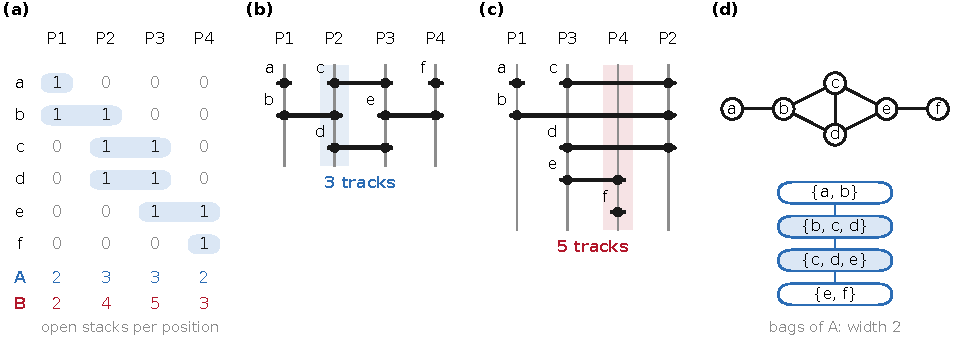
\includegraphics[width=\linewidth]{sec1_fig1_example.pdf}
\caption{One instance, three readings, one number. (a) Six customers and four
patterns, with each customer's open stack shaded in order A; order A keeps at
most 3 stacks open and order B at most 5, and only 2 of the 24 orders reach 3.
(b, c) The same matrix as a gate matrix layout: the same two orders need 3 and
5 tracks (the shaded gate is where the density peaks). (d) The same matrix as a
\emph{graph}, one clique per pattern: the open sets of order A are the bags of a path
decomposition of width 2, so the optimum is the pathwidth plus one
(Theorem~\ref{thm:mosp}).}
\label{fig:example}
\end{figure}

The same matrix is a problem in VLSI design. In a \emph{gate matrix layout}
the patterns are gates, drawn as vertical lines in some order, and the
customers are nets. Each net is a horizontal wire from the first gate it
connects to the last, and wires that overlap must lie on different horizontal
tracks. The task is to order the gates so that the fewest tracks suffice.
Figure~\ref{fig:example}(b) and (c) draw the two orders. The wires are the same;
only the gate order changes which wires overlap. Order A packs into 3 tracks
and order B needs 5. The number of tracks a gate order needs is its
\emph{density}, the most wires crossing any one gate, and that is exactly the
number of open stacks there. So the two problems compute the same number from
the same matrix \citep[Proposition~2]{LY2002}.

The same matrix is also a graph. Make each customer a vertex, and join two
customers when some pattern needs both, so that each pattern becomes a clique
(Figure~\ref{fig:example}(d)). Write down, for order A, the set of open stacks
at each position: $\{a,b\}$, $\{b,c,d\}$, $\{c,d,e\}$, $\{e,f\}$. These sets
cover every vertex and every edge, and each customer appears in a run of
consecutive sets. In graph theory such a sequence is a \emph{path
decomposition}, its sets are \emph{bags}, and its width is the size of its
largest bag minus one. The least width over all path decompositions is the
\emph{pathwidth} of the graph, here 2. The construction works in both
directions, so the fewest open stacks is always the pathwidth plus one
(Theorem~\ref{thm:mosp}).

The same graph is, finally, a sparse symmetric matrix of numerical linear
algebra, with a nonzero wherever two customers share a pattern. The frontal
method eliminates its rows one at a time and must keep in memory the
\emph{wavefront}, the rows already touched but not yet eliminated. Eliminating
the customers in the order $a,b,\dots,f$ keeps at most 3 rows active at once,
and no order does better: the least maximum wavefront is again the pathwidth
plus one (Theorem~\ref{thm:core}). This fourth reading is not in our 2002
table, and we add it below.

\begin{table}[tbp]
\centering
\caption{Twelve problems from three fields, published as one family: eight
rows are exact, counting the pathwidth row itself; two are bands; two are false
as the table states them. Our own table of 2002, reproduced from
\citet[Table~1, p.~1764]{LY2002} with its row order, wording and references as
printed, and its caption: ``Display of a family of equivalent problems studied
independently on the literature''. The shaded column corrects it: it gives the
relation to pathwidth ($\pw$) that is true, proved in Section~\ref{sec:equiv}
(Table~\ref{tab:master}). The last three rows, below the rule, are new:
members of the family that the table missed, which bring a fourth field,
numerical linear algebra.}
\label{tab:ly2002}
\small
\setlength{\tabcolsep}{3.5pt}
\begin{tabular}{@{}lll>{\columncolor{black!7}}l@{}}
\toprule
Problem & Discipline & References & This paper \\
\midrule
MOSP & Operations research & \citet{Yanasse1997b}; \citet{LY2002ref4} & exact: $\pw+1$ \\
Gate matrix layout & VLSI design & \citet{LY2002ref6}; \citet{LY2002ref8} & exact: $\pw+1$ \\
One-dimensional logic & VLSI design & \citet{LY2002ref7} & exact: $\pw+1$ \\
PLA folding & VLSI design & \citet{LY2002ref6} & false$^{a}$ \\
Interval thickness & Graph theory & \citet{LY2002ref5} & exact: $\pw+1$ \\
Node search game & Graph theory & \citet{LY2002ref9} & exact: $\pw+1$ \\
Edge search game & Graph theory & \citet{LY2002ref10} & band: $\pw$ to $\pw+2$ \\
Narrowness & Graph theory & \citet{LY2002ref11} & exact: $\pw+1$ \\
Split bandwidth & Graph theory & \citet{LY2002ref12} & band: $\pw$ to $\pw+1$ \\
Graph path-width & Graph theory & \citet{LY2002ref13} & exact: $\pw$ (reference) \\
Edge separation & Graph theory & \citet{LY2002ref14} & false$^{b}$ \\
Vertex separation & Graph theory & \citet{LY2002ref13} & exact: $\pw$ \\
\midrule
\emph{Progressive pebbling}$^{c}$ & Graph theory & \citet{LY2002ref10} & exact: $\pw+1$ \\
\emph{Vertex search}$^{d}$ & Graph theory & \citet{BRST1991} & exact: $\pw+1$ \\
\emph{Maximum wavefront}$^{e}$ & \begin{tabular}[t]{@{}l@{}}Numerical\\linear algebra\end{tabular} & \citet{KumfertPothen1997} & exact: $\pw+1$ \\
\multicolumn{4}{@{}l@{}}{\footnotesize\emph{New: not in \citet{LY2002}.}} \\
\bottomrule
\multicolumn{4}{@{}p{\linewidth}@{}}{\footnotesize $^{a}$Exact ($\pw+1$) for
multiple folding, with any number of nets per track.
$^{b}$As cutwidth; the vertex separator game of the same reference is exact
($\pw$, for graphs with an edge).
$^{c}$Added by us. Its relation to pathwidth is proved in two papers the table
already cites, for other rows: \citet[Thms~2--3]{LY2002ref14} and
\citet[Thm~3.1]{LY2002ref10}. We prove it in Lean (Appendix~\ref{app:thirteenth}).
$^{d}$Added by us. Searchers occupy vertices and an invisible fugitive moves
along unguarded paths. Exact on every graph with a vertex, edgeless ones
included \citep[(5.1)]{BRST1991}, and equal to node search when the graph has
an edge. We prove it in Lean, following their construction for the upper bound
(Appendix~\ref{app:thirteenth}).
$^{e}$Added by us. The least, over symmetric orderings of a sparse symmetric
matrix with nonzero diagonal, of the largest wavefront
\citep[\S2.1]{KumfertPothen1997}; it is narrowness in another form. The source
defines it but does not state the equality, which we prove in Lean
(Appendix~\ref{app:thirteenth}).}
\end{tabular}
\end{table}

We collected twelve such problems \citep{LY2002}, from operations research,
VLSI design and graph theory, in the table that Table~\ref{tab:ly2002}
reproduces. Each computes, on corresponding inputs, ``a function $f(\Pi)$ that
is either equal to the number of open stacks or closely related to it (plus or
minus one)'' \citep[p.~1764]{LY2002}. The table gives a reference for each
problem, but no proofs and no graph of which problem reduces to which. ``Plus
or minus one'' has two readings. Under the \emph{literal} reading, $f$ is
within one of the number of open stacks on every input. Under the
\emph{fixed-offset} reading, $f$ equals the number of open stacks plus one
constant, the same on every input. Only the second makes solving one problem
the same as solving another. We call the problems that are, on every input,
pathwidth or pathwidth plus one the \emph{pathwidth complex}: most of the
table, and three problems we originally missed. Pathwidth is the quantity
through which every true relation in the table is proved
(Section~\ref{sec:equiv}). It is also the name the literature uses, more than
three times as often as the other eleven names combined (Section~\ref{sec:names}),
so a reader who searches under ``open stacks'' or ``gate matrix layout''
misses most of what is known. The communities that could have checked the
table rarely read each other: of 844 works that cite the table's papers, only
six cite both an open-stacks paper and a graph-theory paper.

The table is ours, and its history explains why no one checked which of its
equalities are true. It was first printed in 2001, in the first author's
doctoral thesis \citep[Table~2.1, p.~13]{Linhares2001}, supervised by the
second author, which proved MOSP NP-hard and equal to gate matrix layout. Its
rows were collected over the years of the doctorate, while reading the
literature of each field. Each came with a reference and nothing else: no
row's relation to open stacks was checked, and no published proof was
restated. The table appeared again, row for row, as Table~1 of \citet{LY2002},
and it has been read since as a statement of equivalence.
\citet{GarciaDeLaBandaStuckey2007}, for instance, credit the speed of their
search in this journal to ``the fact that the problem is fixed parameter
tractable (Linhares and Yanasse 2002)''. When MOSP was set as the first
Constraint Modelling Challenge in 2005, the organisers' report pointed to the
table for the problems equivalent to it, ``including graph path-width'', and
credited the second author with the idea of permuting customers rather than
products \citep{SmithGent2005,Yanasse1997b}, the idea on which Chu and
Stuckey's customer search (Section~\ref{sec:search}) branches. So the table is
already used to justify algorithms, and whether it is true matters. If it is
true, \emph{every result} about any one of the twelve problems transfers to
\emph{all} the others. Looking back, the table was the thesis's most important
finding, and this article does what the thesis did not: it states each problem
precisely, proves what is true and refutes what is not. This paper asks:
\emph{which of the equalities in the Linhares--Yanasse table are true, and what
follows when results, algorithms and benchmarks are moved between the twelve
problems through pathwidth?}

\paragraph{Three more members.} The table was also incomplete. Progressive
pebbling, a game in which pebbles are placed on the vertices of a graph and
each vertex is pebbled once, needs exactly pathwidth plus one pebbles
\citep[Thm~3.1]{LY2002ref10}, and Lengauer's black-white pebbling of a
directed acyclic graph equals the pathwidth of its undirected version plus one
\citep[Thm~2]{LY2002ref14}. Both theorems are in papers that the table
already cites, for its edge-search and edge-separation rows, yet pebbling
itself is not among its problems. \citet[(5.1)]{BRST1991} search for a fugitive
who hides in the vertices, not the edges, and need exactly pathwidth plus one
searchers on every graph with a vertex, including the edgeless graphs where the
table's node search row fails. From numerical linear algebra, the wavefront of
the frontal method, met above \citep[\S2.1]{KumfertPothen1997}, is the problem
of the table: the least maximum wavefront is the pathwidth of the matrix's
graph plus one, on every nonempty matrix. We add the three as the last rows of
Table~\ref{tab:ly2002}, marked as new, and prove all three relations in the
Lean proof assistant (Appendix~\ref{app:thirteenth}). For pebbling and the
vertex search, what is new is the membership: the equivalences were published,
but the table did not include them. For the wavefront the equality itself is
ours: it is elementary, as the wavefront is narrowness read in another form,
but no source we have read states it.

\paragraph{What we find.}
\begin{itemize}
\item \emph{The table, settled.} Eight of the twelve rows are exact: on every
  input, outside degenerate cases such as an empty graph, the problem equals
  pathwidth or pathwidth plus one (the pathwidth row itself is one of the
  eight). Two rows, split bandwidth and edge
  search, lie in \emph{bands}: within one and two of pathwidth, but not at a
  fixed offset. Two rows, PLA folding and edge
  separation, are false as stated, with counterexamples. A variant of each
  false row is exact. Three problems outside the table are exact members
  too: progressive pebbling, a vertex search, and the maximum wavefront of
  sparse matrix elimination (Section~\ref{sec:equiv}).
\item \emph{One name.} The literature has settled on ``pathwidth'', which has
  more than three times as many relevant works as the other eleven names
  combined. Since 2005, after pathwidth, the most active name of the twelve is
  MOSP, and the best exact search for the whole family came from that
  community, by way of the 2005 Constraint Modelling Challenge
  (Section~\ref{sec:names}).
\item \emph{Two false theorems, and our correction.} The best exact algorithm
  for MOSP, the \emph{customer search} of \citet{ChuStuckey2009}, which we call
  the previous algorithm, branches on the order in which customers' stacks
  close, and it is also a pathwidth algorithm. We prove in Lean, however, that
  two of its published dominance theorems, the \emph{definite move} and the
  \emph{better move}, are false, as are their later restatements
  \citep{Chu2011,Fink2012}: each can discard the last remaining solution at a
  node of the search tree. We provide a counterexample instance: our
  implementation of their algorithm, with its better move off, obtains an
  optimum of 7, while our corrected version obtains 6, provable also by a SAT
  (Boolean satisfiability) solver. This is a theorem checked in Lean: the
  whole run of their algorithm on the instance, and its optimum of 6
  (Theorem~\ref{thm:wrong}). Our corrected
  definite move was also found by Tamaki as a lemma
  \citep[Lemma~1]{Kitsunai2016}, in the exact pathwidth literature; we show
  that it can be tested by one bipartite matching per candidate, and prove our
  corrected search sound. Our correction costs at most 2\% more search nodes
  on each group of benchmarks we measured.
\item \emph{A pathwidth solver.} Ported to graphs, our corrected search is an
  exact pathwidth solver, which we release. Within 600 seconds per graph it
  proves the pathwidth of 11,194 of the 11,534 Rome graphs, a graph-drawing
  benchmark of 10 to 110 vertices; all 50 trees of VSPLIB, a benchmark library
  for vertex separation; and 39 of its 73 Harwell--Boeing graphs, the sparsity
  patterns of engineering matrices. On each set this is as many graphs or more
  than the published branch and bound of \citet{CoudertMazauricNisse2016}
  (Section~\ref{sec:results}).
\item \emph{Benchmarks re-certified, and a dataset.} Our corrected search
  re-proved all 115 benchmark optima, on 113 distinct graphs, that rested on
  the previous algorithm, and none changed. We release 17,714 graphs, distinct
  up to isomorphism, from twenty benchmark collections of MOSP, VLSI layout,
  vertex separation, graph drawing and treewidth; 16,088 have a certified
  pathwidth with a layout that attains it, and so a certified value for every
  problem of the pathwidth complex (Section~\ref{sec:results}).
\end{itemize}

\paragraph{How to read the paper.} Section~\ref{sec:equiv} states the twelve
problems and proves what is true. Section~\ref{sec:names} measures which names
and communities the literature uses. Section~\ref{sec:search} reads the exact
open-stacks search as a pathwidth algorithm, finds the two false rules and
proves our corrected search sound. Section~\ref{sec:results} reports what our
corrected search costs, how it performs as a pathwidth solver, and the dataset, and Section~\ref{sec:closing} returns to the question this paper asks.
Every theorem we state is machine-checked in the Lean~4 proof assistant, unless
the text says otherwise. The
reader need not read Lean: each proof is given or cited in the text, and
Appendix~\ref{app:lean} maps each result to its formal statement.
Appendix~\ref{app:machinery-all} holds the supporting material,
and Appendix~\ref{app:names} the bibliometric method. The Lean development,
both solvers, the dataset and an independent checker for each are openly
available, the code and proofs as open source under the MIT licence
(page~\pageref{sec:data}).

% Section 2 (was Section 3 before loop0009 item 01; rewritten for readability
% in item 03). Sources: paper1/problem_transformations.md (problems,
% statements, proofs), paper1/equivalences.md (master table, sources, gaps),
% paper1/proof_reductions.md (faults in published proofs). Lean:
% lean/MOSPFormalization/ and Complex/; axioms printed by paper1/axiom_check.lean.
% Lean names in Appendix A; formal definitions of the eight problems of
% Table 2.1, the old 3.3 and the old 3.4 are in Appendix B. The band end
% values (K_2, K_{1,3}, K_{3,3}) are computed by paper1/complex_check.py
% (equivalences.md, "Not formalised, by choice").
\section{The equivalences, proved}
\label{sec:equiv}

This section answers the first half of our question: which rows of the
Linhares--Yanasse table are true, and in what sense. Section~\ref{sec:intro}
separated two readings of ``plus or minus one''. We call a row \emph{exact}
when it meets the fixed-offset reading: its value is pathwidth, or pathwidth
plus one, on every input. We call it a \emph{band} when it meets only the
literal reading: its value stays within a fixed distance of pathwidth, and
both ends of that range occur. We call it \emph{false} when it meets neither.
The answer is that eight rows are exact, two are bands and two are false.
Section~\ref{sec:problems} states the problems. Section~\ref{sec:true} proves
the answer in four steps: the hub theorem, which ties MOSP to pathwidth; the
other exact rows; the bands; and the false rows. Table~\ref{tab:master} and
Figure~\ref{fig:chain} summarise it.

All theorems below are verified in the Lean proof assistant, unless the text
says otherwise; Appendix~\ref{app:lean} lists the formal statements. Where a
result is published, we cite the published proof and do not repeat it.

\paragraph{Notation.} Table~\ref{tab:notation} lists the symbols used in the
rest of the paper. Graphs are finite and simple. A 0/1 matrix $M$ has the
customers as rows and the patterns as columns; in the VLSI problems the rows
are nets and the columns gates. Row $r$ is \emph{active} at position $j$ of a
column order $\pi$ if it has 1s in two columns $x,y$ with
$\pi(x)\le j\le\pi(y)$, possibly $x=y$: its stack is open there. ``$M$ has a
1'' excludes only the all-zero matrix. One letter needs care. In this section
$k$ is the bound in each decision problem, so for pathwidth it bounds a width.
In Section~\ref{sec:search} $k$ bounds the number of open stacks, which is one
more than a width; we say so again there.

\begin{table}[tbp]
\centering\small
\caption{Notation. Each symbol has one meaning throughout the paper; the
symbols of the search are defined in Section~\ref{sec:search-def}.}
\label{tab:notation}
\begin{tabularx}{\linewidth}{@{}>{\raggedright}p{3.2cm}>{\raggedright\arraybackslash}X@{}}
\toprule
Symbol & Meaning \\
\midrule
$G=(V,E)$, $n=|V|$ & a graph, its vertices and edges; in Section~\ref{sec:search} the vertices are the customers, $V=C$ \\
$L$ & a \emph{layout}, a bijection $V\to\{1,\dots,n\}$ \\
$X_1,\dots,X_r$ & the bags of a path decomposition \\
$M$; $C$; $P$ & a 0/1 matrix; its rows (customers, nets); its columns (patterns, gates) \\
$G_M$ & the \emph{MOSP graph}: vertex set $C$, two customers adjacent when some pattern has a 1 in both rows; each pattern becomes a clique \\
$H$ & the \emph{net graph} of a circuit: two nets adjacent when they share a gate \\
$\pi$ & an order of the columns \\
$Z(M)$, $t(M)$ & the MOSP value (fewest open stacks) and the gate matrix layout value (fewest tracks) \\
$\pw$, $\vs$ & pathwidth and vertex separation \\
$\theta$, $\ns$, $\mns$, $\es$, $\pes$, $\nu$, $\sbw$, $\cw$, $\mcw$, $\VSG$, $\pla$ & the values of the other problems (Table~\ref{tab:problems}) \\
$k$ & the bound of a decision problem; in Section~\ref{sec:search}, a bound on open stacks, so width $k-1$ \\
$w$ & a width, as in ``pathwidth $w$'' \\
$N[c]$ & the closed neighbourhood of $c$: $c$ and its neighbours \\
$\partial T$, $b(T)$ & the border of a vertex set $T$, the vertices outside $T$ with a neighbour in $T$; $b(T)=|\partial T|$ \\
\bottomrule
\end{tabularx}
\end{table}

\subsection{The problems}
\label{sec:problems}

Each problem is a decision problem with an instance and an integer $k$; its
value is the least $k$ for which the answer is yes. Four of the twelve carry
the rest of the paper, and we define them in full. Figure~\ref{fig:example}
shows each on one instance.

\begin{description}
\item[Pathwidth $\pw(G)$.] Is there a sequence of bags $X_1,\dots,X_r\subseteq V$
  covering $V$, with every edge inside some bag, $X_i\cap X_\ell\subseteq X_j$
  whenever $i\le j\le\ell$, and $|X_i|\le k+1$? \citep[p.~346]{LY2002ref13}.
  The condition on $X_i\cap X_\ell$ is the \emph{interval property}: the bags
  that contain a vertex are consecutive.
\item[Vertex separation $\vs(G)$.] Is there a layout $L$ such that for every
  $i<n$ at most $k$ vertices $u$ with $L(u)\le i$ have a neighbour $v$ with
  $L(v)>i$? \citep[p.~346]{LY2002ref13}.
\item[MOSP $Z(M)$.] Given a 0/1 matrix $M$ of customers by patterns, is there
  an order of the patterns with at most $k$ customers active at every position?
  \citep[eqs.~(1)--(2)]{LY2002}.
\item[Gate matrix layout $t(M)$.] Given a net--gate matrix, is there an order of
  the gates and an assignment of nets to $k$ tracks such that nets active at a
  common position get different tracks? \citep[p.~18]{LY2002ref6};
  \citep[Problem~1]{LY2002ref8}.
\end{description}

The other eight problems are needed only to read the table.
Table~\ref{tab:problems} gives each in one line; Appendix~\ref{app:defs} gives
the formal definitions, with the sources.

\begin{table}[tbp]
\centering\small
\caption{The other eight problems of the Linhares--Yanasse table look
unrelated (two circuit layouts, two search games and four graph problems), yet
each asks for the least $k$ that is possible. One line each. Formal definitions are in
Appendix~\ref{app:defs}.}
\label{tab:problems}
\begin{tabularx}{\linewidth}{@{}>{\raggedright}p{3.6cm}>{\raggedright\arraybackslash}X@{}}
\toprule
Problem & In one line \\
\midrule
One-dimensional logic & Order the gates of a circuit so that the intervals
  spanned by the nets overlap at most $k$ at any point. Its graph is the
  \emph{net graph} $H$, which joins two nets that share a gate. A boundary
  variant pins two gates to the ends. \\
PLA folding $\pla(M)$ & Gate matrix layout in at most $k$ tracks, with at most
  two nets on a track. With no limit per track (\emph{multiple folding}) it is
  gate matrix layout itself. \\
Interval thickness $\theta(G)$ & Add edges to $G$ to make an interval graph
  whose largest clique has at most $k$ vertices. \\
Node search $\ns(G)$ & Searchers are placed on and removed from vertices. An
  edge is cleared when both its ends hold a searcher, and becomes contaminated
  again if a searcher-free path joins it to a contaminated edge. Clear every
  edge with at most $k$ searchers at once. $\mns(G)$ is the same with no
  recontamination allowed. \\
Edge search $\es(G)$ & Node search with a third move: sliding a searcher along
  an edge clears it. $\pes(G)$ is the same over \emph{progressive} strategies,
  which never recontaminate an edge. \\
Narrowness $\nu(G)$ & Add the vertices one at a time in some order, and drop
  each as soon as all its neighbours have been added. Never hold more than $k$. \\
Split bandwidth $\sbw(G)$ & Repeatedly split a vertex into an edge, sharing its
  neighbours between the two ends, so that the result has a layout in which
  adjacent vertices are at most $k$ apart (its \emph{bandwidth}). \\
Edge separation & The table's reference \citep{LY2002ref14} supports three
  readings: cutwidth $\cw(G)$, the most edges crossing a gap of a layout;
  modified cutwidth $\mcw(G)$, the most edges passing strictly over a vertex;
  and Lengauer's vertex separator game $\VSG(G)$, a pebbling game that counts
  the unpebbled vertices adjacent to pebbled ones. \\
\bottomrule
\end{tabularx}
\end{table}

\subsection{What is true}
\label{sec:true}

Table~\ref{tab:master} gives the answer row by row, and
Figure~\ref{fig:chain} draws it as a graph around pathwidth. The rest of this
subsection proves it.

\begin{table}[tbp]
\centering\small
\caption{The Linhares--Yanasse table, settled. Eight rows are exact, two are
bands and two are false, and every true relation is a relation to pathwidth.
\emph{Relation}: what is true and proved in Lean, on the graph the problem
lives on (the MOSP graph or the net graph $H$ for the matrix problems, the input
graph otherwise). \emph{Published source}: the published work the row rests on; the
Lean proofs are listed in Appendix~\ref{app:lean}. \emph{Status}: \emph{exact}, a fixed
offset; \emph{band}, an inequality whose ends both occur; \emph{false}, the
table's claim fails, with a counterexample family proved in Lean.}
\label{tab:master}
\begin{tabularx}{\linewidth}{@{}>{\raggedright}p{2.7cm}>{\raggedright}p{3.4cm}>{\raggedright\arraybackslash}X l@{}}
\toprule
Problem & Published source & Relation & Status \\
\midrule
MOSP & \citet{Yanasse1997a}; \citet{FellowsLangston1989}; \citet{LY2002} &
  $Z(M)=\pw(G_M)+1$ ($M$ has a 1) & exact \\
Gate matrix layout & \citet{LY2002ref6} & $t(M)=Z(M)=\pw(G_M)+1$ & exact \\
One-dim.\ logic & \citet{LY2002ref7} & tracks $=\theta(H)=\pw(H)+1$; boundary variant $\ge\pw(H)+1$ & exact \\
PLA folding & \citet{LY2002ref6} & $\max(\pw+1,\lceil|C|/2\rceil)\le\pla$, gap unbounded; multiple folding $=\pw+1$ & false; variant exact \\
Interval thickness & \citet{LY2002ref6}; \citet{LY2002ref9} & $\theta=\pw+1$ ($V\ne\emptyset$) & exact \\
Node search & \citet{LY2002ref9,LY2002ref10}; \citet{BienstockSeymour1991} & $\ns=\mns=\vs+1=\pw+1=\theta$ ($E\ne\emptyset$) & exact \\
Edge search & \citet{EllisSudboroughTurner1994}; \citet{LY2002ref10} & $\vs\le\es\le\vs+2$, also for $\pes$ & band \\
Narrowness & \citet{LY2002ref11} & $\nu=\pw+1$ ($V\ne\emptyset$) & exact \\
Split bandwidth & \citet{LY2002ref12} & $\pw\le\sbw\le\pw+1$ & band \\
Pathwidth & \citet{LY2002ref13} & the reference & exact \\
Edge separation$^{a}$ & \citet{LY2002ref14} & $\cw,\mcw$ unbounded against $\pw$ (stars); $\VSG=\max(1,\vs)$ & false; VSG exact \\
Vertex separation & \citet{LY2002ref13} & $\vs=\pw$ & exact \\
\midrule
\multicolumn{4}{@{}l@{}}{\emph{Not in the Linhares--Yanasse table}} \\
Progressive pebbling & \citet{LY2002ref14}; \citet{LY2002ref10} & $\mathrm{mpb}=\pw+1$ ($V\ne\emptyset$), $=\ns$ ($E\ne\emptyset$) & exact \\
Vertex search & \citet{BRST1991} & $=\pw+1$ ($V\ne\emptyset$), $=\ns$ ($E\ne\emptyset$) & exact \\
Maximum wavefront & \citet{KumfertPothen1997} & $\min\mathrm{wf}=\pw+1=\nu$ (matrix nonempty) & exact \\
\bottomrule
\multicolumn{4}{@{}p{\linewidth}@{}}{\footnotesize $^{a}$Also misattributed:
what \citet{LY2002ref14} proves exactly is the vertex separator game, which is
the table's vertex separation row.}
\end{tabularx}
\end{table}

\begin{figure}[tbp]
\centering
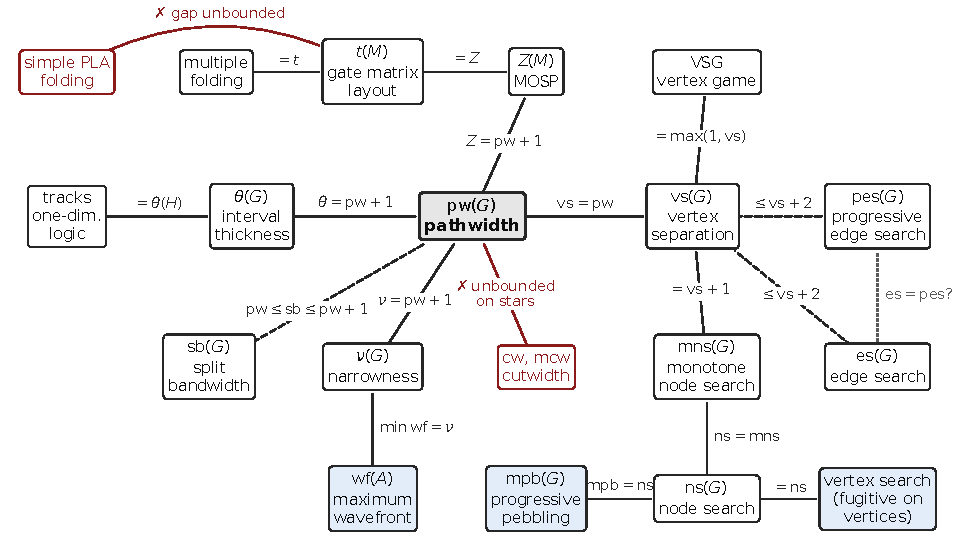
\includegraphics[width=\linewidth]{sec3_fig1_chain}
\caption{Pathwidth is the hub of the table: every exact relation is one or two
steps from it, and the only failures are the two false claims, in dark red. Solid edges are exact relations and dashed edges bands, both
proved in Lean; the dotted edge is LaPaugh's $\mathrm{es}=\mathrm{pes}$, the
one relation not proved, which no row needs. Each false claim is refuted by a
counterexample family proved in Lean. The four matrix problems (top left) live
on the MOSP graph $G_M$ or the net graph $H$. Hypotheses are omitted: $M$ has
a 1, $V\neq\emptyset$, or $G$ has an edge, as in Table~\ref{tab:master}. Two
edges that follow from the others, $\mathrm{mns}=\theta$ and
$\mathrm{ns}=\mathrm{vs}+1$, are not drawn. The shaded nodes on the bottom
row are members the table missed. The vertex search edge holds whenever $G$
has an edge, and the vertex search is $\pw+1$ on every graph with a vertex
\citep[(5.1)]{BRST1991}~\leanref{vsearch}.}
\label{fig:chain}
\end{figure}

\paragraph{The hub.} Two theorems tie the table to pathwidth. The first joins
the two graph rows, vertex separation and pathwidth. The second joins MOSP to
pathwidth, and through it all four matrix problems. The second rests on one
lemma about path decompositions. For a vertex $v$, let $\mathrm{first}(v)$ and
$\mathrm{last}(v)$ be the least and greatest indices of bags containing $v$; by
the interval property, $v\in X_i$ exactly when
$\mathrm{first}(v)\le i\le\mathrm{last}(v)$.

\begin{lemma}[cliques sit in a bag]\label{lem:clique}
In a path decomposition of $G$, every clique of $G$ lies inside one bag~\leanref{clique}.
\end{lemma}
\begin{proof}
The bags containing a vertex $u$ of the clique form the interval
$[\mathrm{first}(u),\mathrm{last}(u)]$. Two vertices of the clique are
adjacent, so their edge lies in a bag and their intervals meet. Pairwise
intersecting intervals of a line have a common point (the Helly property): let
$a$ be the largest left end; every right end is at least every left end, so at
least $a$, and $a$ lies in all of them. So all the intervals share an index
$i$, and the clique lies in $X_i$.
\end{proof}

The first theorem is known. It says the two graph rows of the table are the
same quantity.

\begin{theorem}[vertex separation is pathwidth; known]\label{thm:vs}
For every graph, $\vs(G)=\pw(G)$~\leanref{vs}.
\end{theorem}
This is Theorem~3.1 of \citet{LY2002ref13}. Both directions are constructions.
From a layout of separation $k$, each bag is the set counted at a cut together
with the next vertex. From a decomposition, ordering the vertices by
$\mathrm{first}$ gives a layout of the same width.

The second theorem is the one the rest of the paper uses. In
Figure~\ref{fig:example}(d), the sets of customers active at each step of the
good order are the bags of a path decomposition of the MOSP graph. The theorem
says that this always works, in both directions.

\begin{theorem}[MOSP is pathwidth plus one]\label{thm:mosp}
If $M$ has a 1, then $Z(M)=\pw(G_M)+1$~\leanref{mosp}.
\end{theorem}
\begin{proof}
($\le$) Take a decomposition of $G_M$ of width $k$. The rows of each column $p$
form a clique, so by Lemma~\ref{lem:clique} they lie in a bag $X_{\beta(p)}$.
Order the columns by $\beta(p)$. If row $r$ is active at the position of column
$p$, it has columns $x,y$ with $\beta(x)\le\beta(p)\le\beta(y)$, and
$r\in X_{\beta(x)}\cap X_{\beta(y)}$, so the interval property gives
$r\in X_{\beta(p)}$. At most $k+1$ rows are active there.

($\ge$) Take an order with at most $Z=Z(M)$ active rows at every position. The
active sets, with a singleton bag for each row with no 1, form a path
decomposition: rows sharing a column are both active at its position, and a row
is active on an interval of positions. Its width is $Z-1$, using $Z\ge1$.
\end{proof}
An independent, graph-theoretic route to the same equality is Theorem~2 of
\citet{SuchanTodinca2007}: every minimal interval completion of a graph with an
edge clique cover is obtained by ordering the cover's cliques, and a MOSP
matrix's patterns are such a cover of $G_M$.
For the table, this settles the MOSP row as exact, with offset one, on the MOSP
graph. Read as a cutting problem, Theorem~\ref{thm:mosp} is Proposition~5 of
\citet{Yanasse1997a}, which turns each pattern into a clique on its piece types.
Read as a layout problem, it is Theorem~7 of \citet{FellowsLangston1989}, with
the column-expansion Lemma~4.1 of \citet{FellowsLangston1987}.
\citet[Prop.~2]{LY2002} identify MOSP with gate matrix layout. The proof above
needs no assumption that the instance is reduced.

The graph matters. The MOSP literature also uses a second graph, with the
patterns as vertices, joined when they share a customer, to split an instance
into independent parts \citep{YanasseSenne2010}. It is natural to expect its
pathwidth to measure the open stacks as well; it does not, in either
direction. One pattern shared by four customers who each have a private
pattern has $Z=4$, while its pattern graph is the star $K_{1,4}$, of
pathwidth~1~\leanref{star}. A single customer with many patterns errs the
other way.

\paragraph{The exact core.} The other exact rows attach to
Theorems~\ref{thm:vs} and~\ref{thm:mosp} by published arguments. We do not
reprove them on paper; each item below cites the published proof, and the Lean
proofs are listed in Appendix~\ref{app:lean}. We call the problems that equal
pathwidth or pathwidth plus one on every input the \emph{exact core}, the
members of the pathwidth complex of Section~\ref{sec:intro}: the eight exact
rows, with multiple folding and the vertex separator game, and the three
members outside the table (Appendix~\ref{app:thirteenth}), thirteen problems,
or twelve if multiple folding is counted with gate matrix layout, which it
equals.

\begin{theorem}[the exact core]\label{thm:core}
\leavevmode
\begin{enumerate}
\item Gate matrix layout is MOSP on the same matrix: if $M$ has a 1,
  $t(M)=Z(M)=\pw(G_M)+1$. For a fixed gate order the fewest tracks equals the
  most nets active at one position, by the left-edge algorithm
  \citep[p.~31]{LY2002ref6}~\leanref{core-gml}.
\item Interval thickness: if $V\ne\emptyset$, $\theta(G)=\pw(G)+1$
  \citep[Prop.~3.5]{LY2002ref6}~\leanref{core-it}.
\item One-dimensional logic: if every net meets at least one gate, the
  fewest tracks is $\theta(H)$; if at least one net meets a gate (the matrix
  has a 1), it is $\pw(H)+1$
  \citep[Thm~3]{LY2002ref7}~\leanref{core-logic}.
\item Narrowness: if $V\ne\emptyset$, $\nu(G)=\pw(G)+1$, and for each order
  $\sigma$, $\nu(\sigma)=\vs(\sigma^{\mathrm{rev}})+1$
  \citep[Prop.~3.1]{LY2002ref11}~\leanref{core-narrow}.
\item Node search: for every graph $\ns(G)=\mns(G)$, and if $E\ne\emptyset$,
  $\ns(G)=\vs(G)+1=\pw(G)+1=\theta(G)$
  \citep[Thm]{LY2002ref9}; \citep[Thms~2.3, 4.1]{LY2002ref10}~\leanref{core-ns}.
\item Multiple folding: the fewest tracks is $t(M)=\pw(G_M)+1$
  \citep[Thm~3.14]{LY2002ref6}~\leanref{core-fold}.
\item Lengauer's vertex separator game: $\VSG(G)=\max(1,\vs(G))$
  \citep[Thm~4]{LY2002ref14}~\leanref{core-vsg}.
\item Progressive pebbling: if $V\ne\emptyset$, $\mathrm{mpb}(G)=\pw(G)+1$
  \citep[Thm~3.1]{LY2002ref10}~\leanref{pebbling}.
\item Maximum wavefront: for a symmetric matrix with nonzero diagonal and graph
  $G$, $V\ne\emptyset$, the least maximum wavefront is $\pw(G)+1=\nu(G)$, and
  for each order the maximum wavefront is $\vs$ of that order plus
  one~\leanref{wavefront}.
\item Vertex search: if $V\ne\emptyset$, the least $n$ admitting a successful
  search of \citet[\S5]{BRST1991} with every $|X_i|\le n$ is $\pw(G)+1$,
  whether or not the search is monotone, and it equals $\ns(G)$ when $G$ has an
  edge \citep[(5.1)]{BRST1991}~\leanref{vsearch}. The formal proof follows
  theirs for the upper bound; for the lower bound, where they use blockages,
  it reduces to node search.
\end{enumerate}
\end{theorem}
For the table, this makes the gate matrix layout, one-dimensional logic,
interval thickness, node search and narrowness rows exact, and gives an exact
variant of each false row. A single certified pathwidth therefore answers
every problem in the exact core; Section~\ref{sec:dataset} uses this.

\paragraph{Bands.} Two rows are not fixed offsets of pathwidth, but stay within
a fixed distance of it.

\begin{theorem}[bands]\label{thm:bands}
For every graph, $\pw(G)\le\sbw(G)\le\pw(G)+1$ \citep[Thm~8]{LY2002ref12}, and
$\vs(G)\le\es(G)\le\vs(G)+2$, and the same for $\pes$
\citep[Thm~2.1]{EllisSudboroughTurner1994}~\leanref{bands}.
\end{theorem}
Every end of both bands occurs. $K_2$ has $\sbw=\pw=1$ and $\es=\vs=1$; the star
$K_{1,3}$ has $\pw=1$ and $\sbw=2$, and $\vs=1$ with $\es=2$; and $K_{3,3}$ has
$\vs=3$ with $\es=5$. These values are computed by brute force from each
quantity's definition, not proved in Lean.\footnote{$\sbw(K_{1,3})\ge2$ is
also argued by hand: splits of a tree are trees and keep at least three
leaves.} \citet{LY2002ref12} assumes a connected graph with at least two
vertices; the Lean proof needs neither. LaPaugh's equality $\es=\pes$
\citep{LaPaugh1993} is the one relation we state and do not prove, and no row
needs it.

For the table, this means the following. Relative to the number of open
stacks $Z=\pw+1$, split bandwidth lies in $[Z-1,Z]$ and edge search in
$[Z-1,Z+1]$. Both stay within one of $Z$, so they meet the literal reading of
``plus or minus one''. Since both ends occur, neither is a fixed offset, so
neither meets the fixed-offset reading.

\paragraph{False rows.} Two rows fail even the literal reading: no constant
bounds their distance from pathwidth.

\begin{theorem}[two rows are false]\label{thm:false}
\leavevmode
\begin{enumerate}
\item PLA folding: for a matrix with a 1 and net set $C$,
  $\max(\pw(G_M)+1,\lceil|C|/2\rceil)\le\pla(M)$, and the gap to $\pw+1$ is
  unbounded. The $5\times5$ identity needs 3 tracks while $\pw(G_M)+1=1$, and the
  path $P_n$ as a matrix, one gate per edge, has $t=2$ and
  $\pla\ge\lceil n/2\rceil$, so the gap is unbounded on connected instances too
  \citep[Prop.~3.15]{LY2002ref6}~\leanref{false-pla}.
\item Edge separation read as cutwidth: $\pw\le\cw$ always, but
  $\cw(K_{1,n})\ge n/2$ and $\mcw(K_{1,n})\ge n/2-1$ while $\pw(K_{1,n})=1$; so
  neither cutwidth reading is within a constant of pathwidth~\leanref{false-cw}.
\end{enumerate}
\end{theorem}
For the table, these rows are false as stated. Each has an exact variant
(Theorem~\ref{thm:core}): the PLA claim holds for multiple folding, and the
edge-separation reference proves exactly the vertex separator game.

Several published equalities need a nondegeneracy hypothesis, and one published proof has a gap that we correct; Appendix~\ref{app:edge} gives the details.
Appendix~\ref{app:thirteenth} adds three problems outside the table to the
exact core.

\paragraph{Summary.} Eight of the twelve rows of the Linhares--Yanasse table
are exact, counting the pathwidth row itself, which is the reference. The other
seven are pathwidth, or pathwidth plus one, exactly: MOSP, gate matrix layout,
one-dimensional logic, interval thickness, node search, narrowness and vertex
separation. So are two variants of the false rows, multiple folding and
Lengauer's vertex separator game. Split bandwidth and edge search are bands of
width one and two, within one of the number of open stacks but not at a fixed
offset. Simple PLA folding and edge separation are false as stated. Three
problems the table does not list are exact as well: progressive pebbling, the
vertex search of \citet{BRST1991}, and the maximum wavefront of
\citet{KumfertPothen1997}. One theorem is stated and not proved, LaPaugh's
$\es=\pes$, and no row needs it.
One of the table's references, Kashiwabara and Fujisawa (1979), is one we could not obtain; its
row is proved from \citet{LY2002ref6} and \citet{LY2002ref9}.

% Section 3, rewritten in loop0009 item 04 (review change 7; the owner's notes).
% Sources: paper1/popularity.md ("For the paper"), the numbers of
% paper1.section2_figures.numbers() (OpenAlex caches of 2026-09-29), the period
% counts of paper1.trends.binned, Chu & Stuckey (2009) section 1
% (literature/chu_stuckey_2009.pdf, pp. 2-3), and the graph benchmark counts of
% paper1/solver_fix.md ("Table 1: proved widths", repaired rules) against
% Coudert, Mazauric & Nisse (2016) as recorded in
% pathwidth_solver/bench/reference.py. Tables from tables/ (make_tables.py).
% The method detail, the timeline and the full names table are Appendix C.
\section{Why \emph{pathwidth}: the names and the communities}
\label{sec:names}

Section~\ref{sec:equiv} showed that eight of the twelve rows of the
Linhares--Yanasse table are one quantity. A result proved under any of their
names therefore holds under all of them. But a reader who searches under one
name will not find a result published under another. This section asks two
questions about the literature. Which name does it use for the quantity? And,
besides that name, which community has been most active? The answers are
pathwidth, by far (Figure~\ref{fig:names}), and open stacks
(Table~\ref{tab:periods}). The second answer explains where the best
exact algorithm for the family came from, and leads to Section~\ref{sec:search}.

\paragraph{How we counted.} We searched OpenAlex \citep{Priem2022} on
29 September 2026 for each problem's name and its common variants, in titles and
abstracts, within Computer Science, Mathematics, Engineering and Decision
Sciences. A search hit need not use the name in the table's sense: ``narrowness''
matches term rewriting, and ``path-width'' matches roads and tool paths. So we
read the 2,271 hits and kept the 1,593 that are about one of the twelve problems.
The 700 hits for the eleven smaller names were judged one by one, by one
annotator with model assistance; the 1,571 pathwidth hits were filtered by a
stated rule, checked on samples. A mechanical phrase rule agrees with the
judgements on 78\% of the 700 and leads to the same conclusions. The counts are
lower bounds, since a work can study a problem without naming it in its
abstract. Appendix~\ref{app:names} gives the method in full, the robustness
check and the counts per name. The census covers the twelve names of the
table. The three members we add (Section~\ref{sec:intro}) are not counted:
progressive pebbling and the vertex search are graph-theory names, and the
maximum wavefront belongs to a fourth discipline, numerical linear algebra.

\begin{figure}[H]
\centering
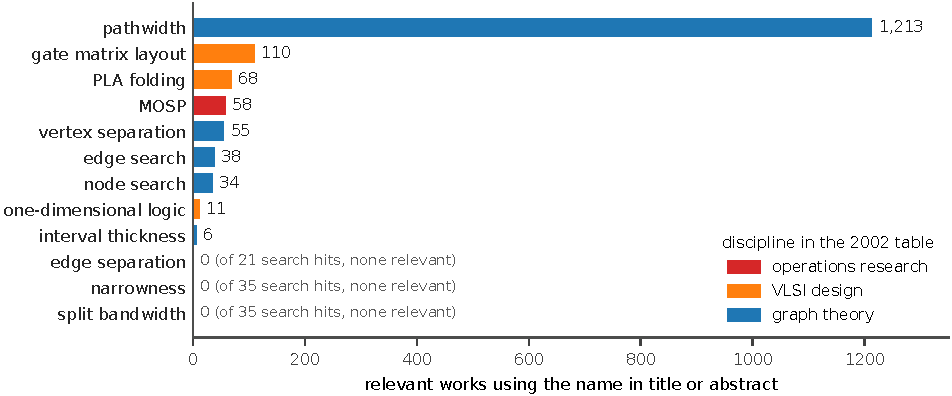
\includegraphics[width=\linewidth]{sec2_fig1_name_usage.pdf}
\caption{Pathwidth has more relevant works than the other eleven names
together, three times over, and three names have none. Works using each
problem's name, in title or abstract, in the sense of the Linhares--Yanasse
table; all years to September 2026. Colour gives the discipline that the table
assigns the problem.}
\label{fig:names}
\end{figure}

\subsection{Pathwidth has absorbed the family}

Figure~\ref{fig:names} gives the counts. Pathwidth has 1,213 relevant works,
21 times as many as MOSP and more than three times as many as the other eleven
names together (380). Three names have no relevant work at all: narrowness,
split bandwidth and edge separation. Two more are rare: interval thickness has
6 works and one-dimensional logic 11. Pathwidth is also the only name still
growing: its 311 works in 2020--2024 are more than the whole history of any
other name (Appendix~\ref{app:names}). So anything one would want to know about
algorithms for this class of problems was most likely published under
``pathwidth''.

\subsection{Besides pathwidth, open stacks}

\begin{table}[t]
\centering\small
\caption{Besides pathwidth, the most active name over 2005--2024 is MOSP,
although vertex separation led in 2015--2019. Relevant works per five-year
period, for the three names with the most works over 2005--2024; the next are
edge search (28) and node search (20).}
\label{tab:periods}
% Generated by python -m paper1.latex.make_tables. Source: paper1.section2_figures.numbers()["periods_2005_24"] (paper1.trends.binned on the OpenAlex trend cache).
% Do not edit by hand.
\begin{tabular}{@{}lrrrrr@{}}
\toprule
Name & 2005--09 & 2010--14 & 2015--19 & 2020--24 & 2005--24 \\
\midrule
Pathwidth & 114 & 179 & 267 & 311 & 871 \\
MOSP & 17 & 17 & 5 & 12 & 51 \\
Vertex separation & 7 & 10 & 15 & 0 & 32 \\
\bottomrule
\end{tabular}
% check: next names over 2005-24: edge search game 28, node search game 20, gate matrix layout 9

\end{table}

The VLSI names belong to the 1980s: since 2005 gate matrix layout has 9
relevant works and PLA folding 6. Table~\ref{tab:periods} shows the
three names with the most works over 2005--2024. MOSP is second, with 51,
ahead of vertex separation (32) and edge search (28). Vertex separation led
only in 2015--2019. The open-stacks community, in operations research, is thus
the one most active besides pathwidth.

\begin{table}[t]
\centering\small
\caption{The open-stacks papers are read apart from graph theory. Works citing
the papers that the Linhares--Yanasse table cites, by the discipline of the
papers they cite. Of 135 works citing an operations-research paper, 6 also cite
a graph-theory paper (4\%); of 285 citing a VLSI paper, 65 do (23\%). The 2002
paper itself counts as operations research. OpenAlex, 29 September 2026; 844
citing works in all.}
\label{tab:communities}
% Generated by python -m paper1.latex.make_tables. Source: paper1.section2_figures.numbers()["discipline_sets"] (OpenAlex citation cache, 2026-09-29).
% Do not edit by hand.
\begin{tabular}{@{}lrrrr@{}}
\toprule
& & \multicolumn{3}{c}{\dots\ of which also cite} \\
\cmidrule(l){3-5}
Works citing & All & operations research & VLSI & graph theory \\
\midrule
operations research & 135 & -- & 14 & 6 \\
VLSI & 285 & 14 & -- & 65 \\
graph theory & 507 & 6 & 65 & -- \\
\bottomrule
\end{tabular}
% check: by set of disciplines cited: GT 438, VLSI 208, OR 117, GT+VLSI 63, OR+VLSI 12, GT+OR 4, GT+OR+VLSI 2; citing works 844

\end{table}

It has also worked largely apart from graph theory. Table~\ref{tab:communities}
counts the 844 works that cite the papers of the table, by the disciplines of
the papers they cite. Only six works cite both an open-stacks paper and a
graph-theory paper. Two are by the table's authors, one is open-stacks work on
graph properties, and three are pathwidth or vertex-separation work from
computer science. The VLSI papers are read with graph theory about five times as
often.

\subsection{From an open-stacks challenge to a pathwidth solver}

It is not a coincidence that the best exact algorithm for MOSP came from the
open-stacks community and is also, on the published evidence, among the
strongest exact algorithms for pathwidth. The account is
in \citet[\S1]{ChuStuckey2009}. MOSP was the subject of the first Constraint
Modelling Challenge \citep{SmithGent2005}, posed in May 2005, which drew 13
entries. The fastest entry, by García de la Banda and Stuckey, combined dynamic
programming with branch and bound and was an order of magnitude faster than
any other \citep{GarciaDeLaBandaStuckey2007}. \citet{ChuStuckey2009} built on
it. They branched on which customer's stack closes next rather than on which
pattern is made next, recorded the states already refuted, added dominance
rules, and became
five to six orders of magnitude faster on hard instances. Their solver closed
every open instance of the challenge within ten seconds. MOSP's busiest decade
in Table~\ref{tab:periods}, 2005--2014, is the decade of this work.

The customer search reads an instance only through its MOSP graph
\citep[p.~4]{ChuStuckey2009}, so it decides pathwidth
(Section~\ref{sec:search}). Ported to graphs, it proves more instances than
reported on the benchmarks where published exact pathwidth results exist, those
of \citet{CoudertMazauricNisse2016}. It proves the pathwidth of 11,194 of the
11,534 Rome graphs (97.1\%), against their 95.6\%, both within 600 seconds per
graph. It proves all 50 VSPLIB trees, against their 30, and 39 of the 73
Harwell--Boeing graphs, against their 26. These are comparisons with published
numbers obtained on other hardware, not a head-to-head run;
Table~\ref{tab:graphs} in Section~\ref{sec:results} gives the full count.

Two consequences shape the rest of the paper. First, a result on any of the
twelve problems should be stated, and searched for, as a result on pathwidth.
Section~\ref{sec:search} does this for the customer search. It finds that the
search's first dominance rule is, in correct form, a theorem already known in
the pathwidth literature, and that two of its published theorems are false.
Second, a benchmark for any problem in the exact core is a pathwidth benchmark,
which is how Section~\ref{sec:dataset} builds its dataset.

% Section 4. Sources: paper1/revised_algorithm.md (4.1-4.6), search_soundness.md,
% prior_art_counterexample.md (prior art). Lean: lean/MOSPFormalization/Search/,
% names in Appendix A (sec9a_appendix_lean.tex). The old 4.6-4.7 are Section 5.
% Restructured 2026-10-06 (loop0009 item 05, review changes 4 and 5): stakes
% first, the pathwidth reading and the dictionary in 4.1, Algorithm 4.1 in 4.2,
% each rule as intuition -> counterexample -> repair -> test.
% Page numbers for Chu & Stuckey (2009) are those of the preprint
% literature/chu_stuckey_2009.pdf; for Chu (2011) the printed ones.
\section{An exact open-stacks search, read as a pathwidth algorithm}
\label{sec:search}

If MOSP is pathwidth (Theorem~\ref{thm:mosp}), then the best exact MOSP
algorithm is a pathwidth algorithm, and its rules can be checked against what
the pathwidth literature knows. This section does that for the \emph{customer
search} of \citet{ChuStuckey2009}, the search that Section~\ref{sec:names}
traced from the open-stacks challenge. It searches over the orders in which the
customers' stacks close, not over pattern sequences, and it prunes with
dominance rules. Three of the rules are stated as theorems (their Theorems~1,
2 and~3) and a fourth, the subset rule, in their \S2. \citet{ChuStuckey2009}
place MOSP among ``graph path-width and gate matrix layout'', citing
\citet{LY2002}, but they do not use pathwidth in the search. Any graph is the
MOSP graph of the instance with one customer per vertex and one pattern per
edge, so the search decides pathwidth for every graph, and ported to graphs,
our corrected search is an exact pathwidth solver, which we release (Sections~\ref{sec:names} and~\ref{sec:results}).

The stakes are these. Two of the published dominance theorems, the
\emph{definite move} and the \emph{better move}, are false, and so are their
restatements in Chu's thesis \citep{Chu2011} and, with a stronger premise, in
\citet{Fink2012}. The error rarely shows: on every benchmark the previous algorithm, the search
as \citet{ChuStuckey2009} publish it, answers correctly, and the only whole
instance we found on which our implementation of it reports a wrong optimum,
with the better move off, has 34 customers. There the \emph{old move}, a rule
that lets a failed sibling prune later branches, passes a false refutation on
(Figure~\ref{fig:wrong}). And when our corrected search re-proved every
benchmark optimum that rested on the previous algorithm, no value changed (Section~\ref{sec:results}). Our corrected definite
move was also found by Tamaki, as the commitment lemma \citep[Lemma~1]{Kitsunai2016},
which says when an exact pathwidth search may commit to one extension of a
vertex set and try no other (Section~\ref{sec:layouts}). We
show that it can be tested by one small bipartite matching per candidate. The
main result, Theorem~\ref{thm:main}, says informally: \emph{with both rules
corrected, the search is sound; whenever it answers that $k$ stacks do not
suffice, they do not, and the graph has pathwidth at least $k$.} Our correction
costs at most 2\% more search nodes on each benchmark set
(Section~\ref{sec:results}).

Section~\ref{sec:search-def} defines the search and shows that it decides
pathwidth, in both vocabularies. Section~\ref{sec:algorithm} gives the
algorithm. Sections~\ref{sec:definite} and~\ref{sec:other-rules} take the
rules one at a time, Section~\ref{sec:theorem} proves our corrected search
sound, and Section~\ref{sec:layouts} places each rule in the pathwidth
literature.

\subsection{The search decides pathwidth}
\label{sec:search-def}

\citet[p.~4]{ChuStuckey2009} observe that the patterns matter only through the
MOSP graph. So fix a graph $G=(C,E)$ whose vertices are the customers, and an
integer $k\ge0$. In this section $k$ bounds the number of open stacks, which is
one more than a width: $k$ stacks suffice exactly when the pathwidth is at most
$k-1$ (Theorem~\ref{thm:decides}). For a customer $c$ write $N[c]$ for its
closed neighbourhood, the stacks that must be open when $c$'s stack closes. For
a set $T\subseteq C$ of vertices, its \emph{border} $\partial T$ is the set of
vertices outside $T$ with a neighbour in $T$. For a set $T$ of closed
customers write
\begin{align*}
O(T) &= \textstyle\bigcup_{c\in T}N[c] && \text{the stacks opened once $T$ has closed},\\
\fin(X) &= \{c : N[c]\subseteq X\} && \text{the customers free to close when $X$ is open},\\
\cl(T) &= \fin(O(T)) && \text{the \emph{free closure} of $T$},\\
b(T) &= |O(T)\setminus T| = |\partial T| && \text{the stacks open after $T$ has closed},\\
o(c,T) &= N[c]\setminus O(T),\quad \open(c,T)=|o(c,T)| && \text{the stacks closing $c$ would newly open.}
\end{align*}
The open stacks after $T$ has closed are exactly the border of $T$, and this
one identity carries the whole translation to pathwidth.

A \emph{move} at $T$ closes one customer $c\notin T$, at cost
$\cost(T,c)=|O(T\cup\{c\})\setminus T| = b(T\cup\{c\})+1$, the stacks open at
that moment counting $c$. It is \emph{playable} when $\cost(T,c)\le k$. Write
$\Ext_k(T)$ (``$T$ extends'') when some order of $C\setminus T$ has every step playable. On entering
a node the search closes every free customer, so it stands only at
\emph{states}, sets with $S=\cl(S)$. The \emph{child} of $S$ by $c$ is
$S\cdot c=\cl(S\cup\{c\})$. The search's predicate $\Sol_k(S)$ holds when
$S=C$, or when some playable $c$ has $\Sol_k(S\cdot c)$~\leanref{defs}. Every
node the search visits satisfies the invariant $b(S)\le k$.

\paragraph{An example.} Take the graph of Figure~\ref{fig:example}(d), with
$k=3$. At $T=\{a\}$ we have $O(T)=\{a,b\}$, so one stack, $b$, is open:
$b(T)=1$ and $\partial T=\{b\}$. No other customer is free, since $N[b]$
contains $c$ and $d$, so $T$ is a state. Closing $b$ newly opens
$o(b,T)=\{c,d\}$ and costs $\cost(T,b)=3$, the stacks $b$, $c$ and $d$; the
move is playable. At $\{a,b,c\}$ every neighbour of $d$ is open, so $d$ is
free, and the child $\{a,b\}\cdot c$ is $\{a,b,c,d\}$. The closing order
$a,b,c,e$ (with $d$ and $f$ closed free) costs $2,3,3,2$, the profile of
order~A in Figure~\ref{fig:example}(a).

\begin{lemma}[free moves never hurt]\label{lem:F}
If $b(T)\le k$, then $\Ext_k(T)\iff\Sol_k(\cl(T))$~\leanref{F}.
\end{lemma}
Closing a customer whose neighbourhood is already open opens nothing, never
makes a later step dearer, and leaves one fewer stack open. The hypothesis is
needed: closing the free customers one by one costs $b(T)$ at each step.

\begin{theorem}[the search decides pathwidth]\label{thm:decides}
For nonempty $C$, $\Sol_k(\emptyset)\iff\pw(G)+1\le k$. On the MOSP graph of an
instance $M$ that has a 1, $\Sol_k(\emptyset)\iff Z(M)\le k$~\leanref{decides}.
\end{theorem}
\begin{proof}
For a closing order $c_1,\dots,c_n$ with prefixes $S_i$, the $i$-th step costs
$1+|\partial S_i|$. Reverse the order to get a layout. Its first $n-i$
vertices are $C\setminus S_i$, and those with a neighbour among the remaining
ones are exactly $\partial S_i$. So the cost of the closing order is the vertex
separation of the reversed layout plus one, and Lemma~\ref{lem:F} at the root
and Theorem~\ref{thm:vs} finish the proof.
\end{proof}

So a refutation, $\neg\Sol_k(\emptyset)$, may only mean $\pw(G)>k-1$. The rest
of the section asks whether the pruning rules preserve that meaning.

\paragraph{In pathwidth language.} The exact pathwidth literature writes
$N(T)$ for the border and $d(T)$ for its size
\citep[p.~390]{KobayashiKomuroTamaki2014}; we keep $\partial T$ and $b(T)$. A
vertex sequence is \emph{$w$-feasible} when every prefix has border at most
$w$, and $\vs(G)$ is the least $w$ for which some permutation is $w$-feasible.
Table~\ref{tab:dictionary} translates each notion of the search into this
vocabulary. Read it row by row: every ingredient of the customer search is a
known ingredient of an exact pathwidth algorithm, and the last two rows are
the rules of Section~\ref{sec:algorithm}.

\begin{table}[t]
\centering\small
\caption{The customer search is, ingredient by ingredient, an exact pathwidth
algorithm: each notion of the search beside its name in the pathwidth
literature. The memo and the definite move are described in
Section~\ref{sec:algorithm}.}
\label{tab:dictionary}
\begin{tabularx}{\linewidth}{@{}>{\raggedright}p{5.2cm}>{\raggedright\arraybackslash}X@{}}
\toprule
Customer search & Layout \\
\midrule
closing order from $\emptyset$ & vertex sequence, read forwards \\
open stacks $b(T)$ & border size $|\partial T|$ \\
$\cost(T,c)$ & $|\partial(T\cup\{c\})|+1$ \\
$\Sol_k(\emptyset)$ & $\vs(G)\le k-1$ \\
free closure $\cl(T)$ & full set of $T$ \citep[p.~328]{SuchanVillanger2009} \\
memo & failure table \\
definite move, corrected & commitment to the child \\
\bottomrule\end{tabularx}
\end{table}

\subsection{The algorithm}
\label{sec:algorithm}

Algorithm~\ref{alg:search} gives the customer search. It is a depth-first
search over states. At each node it closes the free customers, consults a
table of states already refuted, keeps the playable candidates, filters them
with the dominance rules and recurses on the survivors.

\begin{algorithm}[t]
\caption{The customer search \citep{ChuStuckey2009} is a plain depth-first
search; all its pruning sits in the memo (lines~4 and~12), the filter
(line~6) and the old moves (line~9). It decides $\Sol_k(S)$ for a graph
$G=(C,E)$ and a stack bound $k$, and is called as
$\textsc{Search}(\emptyset,\emptyset)$. $Q$ is the set of old moves the node
inherits.}
\label{alg:search}
\small
\begin{tabular}{@{}r@{\quad}l@{\qquad}l@{}}
1 & $\textsc{Search}(S,Q)$: & \\
2 & \quad $S\gets\cl(S)$ & \textcolor{gray}{free moves (Lemma~\ref{lem:F})} \\
3 & \quad \textbf{if} $S=C$ \textbf{then return} true & \\
4 & \quad \textbf{if} $S$ is in the memo \textbf{then return} false & \textcolor{gray}{memo} \\
5 & \quad $A\gets$ the $c\notin S\cup Q$ with $\cost(S,c)\le k$, in index order & \textcolor{gray}{cost cut} \\
6 & \quad $L\gets$ filter of $A$: definite move, then subset rule, then better move & \textcolor{gray}{Sections~\ref{sec:definite}--\ref{sec:other-rules}} \\
7 & \quad $\mathit{seen}\gets Q\setminus S$ & \\
8 & \quad \textbf{for each} $c\in L$: & \\
9 & \quad\quad $Q'\gets\{q\in\mathit{seen} : \cost(S\cup\{q\},c)\le k\}$ & \textcolor{gray}{old moves} \\
10 & \quad\quad \textbf{if} $\textsc{Search}(S\cup\{c\},Q')$ \textbf{then return} true & \\
11 & \quad\quad $\mathit{seen}\gets\mathit{seen}\cup\{c\}$ & \\
12 & \quad add $S$ to the memo & \\
13 & \quad \textbf{return} false & \\
\end{tabular}
\end{algorithm}

Line~2 is safe by Lemma~\ref{lem:F}, and the cost cut of line~5 is exact,
since an unplayable move is not a move of $\Sol_k$. The rest is pruning, and
each piece has a one-sentence intuition.
\begin{itemize}
\item \emph{The memo} (lines~4 and~12): whether a state can be finished does
  not depend on how it was reached, so a state refuted once is refused when
  met again.
\item \emph{Old moves} (lines~7--11): a sibling whose subtree failed stays
  failed further down, as long as closing it first would have kept each later
  step within the bound.
\item \emph{The definite move}: if closing $q$ now leaves no more stacks open
  than before, close $q$ at once and try nothing else
  (Section~\ref{sec:definite} shows why this looks safe and is not).
\item \emph{The subset rule}: if $d$ newly opens a subset of what $r$ newly
  opens, then $d$ is at least as good a move as $r$.
\item \emph{The better move}: if $q$ would be a definite move right after $r$,
  then closing $q$ before $r$ is at least as good as closing $r$ first.
\end{itemize}
Each of the three filtering rules discards a move $r$ by citing a
\emph{covering}, or \emph{link}, from $r$ to a kept move $c$ with
$\Sol_k(S\cdot r)\Rightarrow\Sol_k(S\cdot c)$. The filter runs the definite
move, then the subset rule, then the better move, each once. If the definite
move fires, it keeps its customer alone.

This loop is the decision procedure of \citet[Algorithm~1,
p.~393]{KobayashiKomuroTamaki2014}, which asks whether a vertex set extends to
a $w$-feasible permutation. It has four steps: replace the set by a committed extension, answer
from a failure table or at the full vertex set, recurse on each feasible
one-vertex extension, and record failures. The customer search is that loop
with $w=k-1$. The free closure and the definite move play the part of the
commitment, the memo is the failure table, and the cost cut is the feasibility
test. \citet[\S3.2]{CoudertMazauricNisse2014} has the same three parts in a
branch and bound. Neither line cites the other in the papers we have read:
\citet{ChuStuckey2009} predates the commitments and both 2014 papers, and none
of the pathwidth papers cites it. This is the isolation measured in
Table~\ref{tab:communities}, at the level of one algorithm.

\subsection{The definite move is false as published, and its correction is a matching test}
\label{sec:definite}

The definite move is the strongest of the rules, since when it fires it
discards every other candidate. Its premise looks like a safe accounting:
closing $q$ opens some new stacks and lets some customers close, and if it
lets at least as many close as it opens, nothing seems lost by closing it
first. \citet[\S3.1, p.~6]{ChuStuckey2009} state:
\begin{quote}
\textbf{Theorem 1.} Suppose S ++ [q] is playable and close(q, S) $\ge$
open(q, S), then if U$'$ = S ++ R is a solution, there exists a solution
U = S ++ [q] ++ R$'$.
\end{quote}
Here ++ is concatenation of closing sequences, $R$ and $R'$ are closing
sequences, a \emph{solution} is a complete closing order with every step
playable, and $\close(q,S)$ counts the customers
$d$ with $o(d,S)\subseteq o(q,S)$ (p.~4). The rule keeps $q$ alone. We read $d$
as ranging over customers not yet closed, as our implementation does; read
literally, closed customers count too, which weakens the premise, and both
readings are refuted below. \citet[Thm~6.3.6, p.~142]{Chu2011} restates the
theorem with the same premise and proof, reworded for $k$ stacks. Write
$X=S\cdot q$. The first lemma confirms that the premise says what the
intuition says.

\begin{lemma}[what the premise says]\label{lem:premise}
$\close(q,S)=|X\setminus S|$. Hence the premise holds iff $b(X)\le b(S)$: the
child has no more open stacks than the parent~\leanref{premise}.
\end{lemma}

The premise compares only the two ends, $S$ and $X$. The rule fails because a
set between them can be cheaper still. Figure~\ref{fig:cex}(a) shows the graph on
which it fails, and panel~(b) the cheaper set between.

\begin{counterexample}\label{cex:definite}
Let $G$ be the graph of Figure~\ref{fig:cex}(a), on customers $0,\dots,13$
with 26 edges, and let $S=\{2\}$, $k=6$ and $q=0$. Then $O(S)=\{1,2,3,4\}$,
$o(0,S)=\{0,7,11\}$ and $\cost(S,0)=6$, so $0$ is playable. The customers with
$o(d,S)\subseteq\{0,7,11\}$ are $0$, $3$ and $4$, so $\close(0,S)=3\ge\open(0,S)$,
and $0$ comes first in index order, so the rule keeps only $0$. A solution
exists from $S$: the order
\[1,3,4,6,12,13,0,5,7,8,9,10,11\]
costs at most 6. None exists from the child $X=\{0,2,3,4\}$: only seven sets
are reachable from $X$ by moves of cost at most 6, and none is $C$~\leanref{cex}.
\end{counterexample}

\begin{figure}[t]
\centering
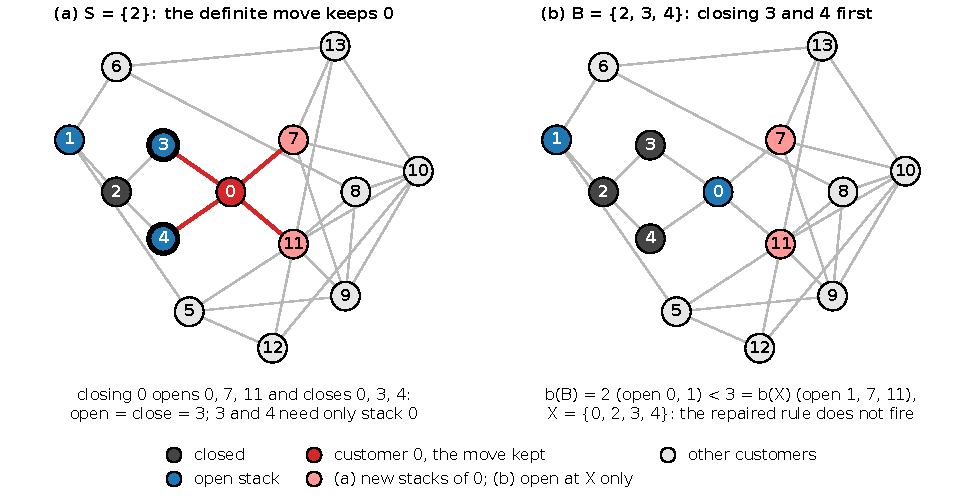
\includegraphics[width=\linewidth]{definite_counterexample.pdf}
\caption{The definite move fails because a set between parent and child is
cheaper than both. (a) The graph of Counterexample~\ref{cex:definite} at the
state where the rule fires. Customer 2 is closed; 1, 3 and 4 are open. Moving 0
opens the new stacks 0, 7 and 11 and closes 0, 3 and 4, so open = close = 3 and
the rule keeps 0 alone. But 3 and 4 have the single new stack 0 between them:
closing them first gains two stacks for the price of one, which a solution
starting with 0 cannot match. (b) The intermediate set $B=\{2,3,4\}$ leaves two
stacks open, fewer than the three of the child $X=\{0,2,3,4\}$, so the corrected
rule of this section does not fire.}
\label{fig:cex}
\end{figure}

The published implication, as a universal statement, is refuted in Lean under
both readings of $\close$, and so is the thesis's Theorem~6.3.6~\leanref{thm1false}.
\citet[pp.~27--28]{Fink2012} restates the rule with a stronger premise,
counting only dominated customers of smaller index than $q$. The graph above
refutes it under no labelling, but a third twin of 3 and 4 gives a
15-customer graph that does~\leanref{fink}. The published proof moves $q$ to
the front of a solution and counts, after each prefix, the stacks $q$ opens
against the customers it lets close. But customers that the solution has
already closed no longer count as closed by $q$, while the stacks $q$ opens may
still be new. Appendix~\ref{app:whyfails} gives the full analysis, and
Appendix~\ref{app:minimality} the search for smaller counterexamples.

\paragraph{The correction.} We require the comparison at every set
between the two ends, not only at $S$. Call $q$ \emph{hereditarily definite} at
$S$ when $b(X)\le b(B)$ for every $B$ with $S\subseteq B\subseteq X$ and
$q\notin B$. By Lemma~\ref{lem:premise}, the published premise is the case
$B=S$. In the counterexample the hereditary condition fails at $B=\{2,3,4\}$
(Figure~\ref{fig:cex}(b)), where
$b(B)=2<3=b(X)$~\leanref{hered}. The proof that the corrected rule is sound needs one
inequality.

\begin{lemma}[open stacks are submodular]\label{lem:submod}
For all $A,B\subseteq C$, $b(A\cup B)+b(A\cap B)\le b(A)+b(B)$~\leanref{submod}.
\end{lemma}
\begin{proof}
$b(T)=|O(T)|-|T|$, $O(A\cup B)=O(A)\cup O(B)$ and $O(A\cap B)\subseteq
O(A)\cap O(B)$; the customers themselves balance exactly.
\end{proof}

\begin{theorem}[the corrected definite move is sound]\label{thm:repaired}
If $q\notin S$ is hereditarily definite at $S$, then $\Ext_k(S)\Rightarrow \Ext_k(X)$.
At a state with the invariant, $\Sol_k(S)\Rightarrow\Sol_k(S\cdot q)$~\leanref{repaired}.
\end{theorem}
\begin{proof}
Take an order from $S$ of cost at most $k$ with prefixes $T_i$, in which $q$ is
the $j$-th step, and follow it from $X$, skipping customers already in $X$. A
step $i<j$ closes $c_i$ at $T_{i-1}\cup X$. We have
$S\subseteq T_i\cap X\subseteq X$ and $q\notin T_i$, so the hypothesis gives
$b(X)\le b(T_i\cap X)$, and Lemma~\ref{lem:submod} gives
$b(T_i\cup X)\le b(T_i)$: the step costs no more than the original. After step
$j-1$ the closed set contains $T_j$ with the same opened set, and the rest of
the order applies. The search's form follows by Lemma~\ref{lem:F}.
\end{proof}

The corrected definite move was also found by Tamaki as a lemma: it is the
commitment lemma of \citet[Lemma~1, p.~142]{Kitsunai2016}, stated there for
directed pathwidth, read on the symmetric digraph with the committed extension
fixed to the child $X=\cl(S\cup\{q\})$. The hereditary premise is their
commitment condition for that extension (Lemma~\ref{lem:endpoint},
Section~\ref{sec:layouts}) and the proof is theirs. The one difference of
statement is that their lemma also assumes that the paths to $S$ and to $X$
stay within budget, which holds at every node the search visits. Both
statements are transcribed in Lean and each is derived from the other under
that assumption; a five-vertex graph shows the assumption is not redundant as
a statement~\leanref{tamaki}.

\paragraph{The matching test.} The corrected rule seems to require checking
exponentially many intermediate sets. It does not, and this cheap test is our
algorithmic contribution in this section; we did not find it in the papers we
hold. In words: the rule is safe exactly when all but one of the new stacks
can be paired with a different freed customer who needed it. In the
counterexample, closing 0 opens three new stacks and frees 3 and 4, both of
whom needed only stack 0: one pairing where two are required.

\begin{theorem}[the corrected premise is a matching condition]\label{thm:matching}
Let $Y=X\setminus(S\cup\{q\})$, and join each $d\in Y$ to the stacks of
$o(d,S)\subseteq o(q,S)$. Then $q$ is hereditarily definite at $S$ iff this
bipartite graph has a matching with at least $\open(q,S)-1$ edges~\leanref{matching}.
\end{theorem}
\begin{proof}
The sets of the hereditary condition are $B=S\cup D$, $D\subseteq Y$, and
$b(X)\le b(S\cup D)$ iff $|D|-|o(D)|\le\delta$ with
$\delta=|Y|+1-\open(q,S)$, where $o(D)$ is the union of the $o(d,S)$. By the
deficiency form of Hall's theorem the largest matching has size
$|Y|-\max_D(|D|-|o(D)|)$, which is at least $|Y|-\delta=\open(q,S)-1$ exactly
when the hereditary condition holds.
\end{proof}

The bipartite graph has at most $\close-1$ customers on one side and $\open$
stacks on the other, and the matching can stop at $\open-1$ edges. Every $q$
with $\open(q,S)\le1$ passes at once, so the definite move of the previous algorithm is right
there~\leanref{open1}.

\subsection{The other rules}
\label{sec:other-rules}

Each of the remaining rules is quoted, proved sound in the form used, and
shown to need the test or tie-break it carries.

\paragraph{The subset rule.} ``If $o(c_i,S)\subseteq o(c_j,S)$ and $i<j$ \dots\
move $j$ can be removed'' \citep[\S2, p.~5]{ChuStuckey2009}. As implemented,
$d$ dominates $r$ when $o(d,S)\subseteq o(r,S)$ and the inclusion is strict or
$d<r$. Every dominated playable $r$ is dropped, with a fallback that keeps $A$
if all would go. The covering is sound for every set $S$: if
$o(d,S)\subseteq o(r,S)$ and $r$ is playable, then $d$ is playable and
$\Sol_k(S\cdot r)\Rightarrow \Sol_k(S\cdot d)$, because $d$ is free after $r$
and closing $d$ then $r$ reaches the same state at no greater cost. With the
index tie-break, domination is a strict order, so an undominated move with a
solution survives, and the fallback never fires when a solution
exists~\leanref{subset}. The tie-break is necessary: without it, two customers
with equal new stacks dominate each other and both go, which loses a solution
on a 7-customer graph~\leanref{tiebreak}.

\paragraph{The better move.} \citet[\S3.2, p.~6]{ChuStuckey2009}: ``Suppose
S ++ [q] and S ++ [r, q] are playable and close(q, S $\cup$ \{r\}) $\ge$
open(q, S $\cup$ \{r\}) then if U$'$ = S ++ [r] ++ R is a solution there exists a
solution U = S ++ [q] ++ R$'$.'' Its premise is the definite move's premise for
$q$ at the child $\cl(S\cup\{r\})$, together with playability of $r$ then $q$,
and its conclusion swaps $q$ and $r$~\leanref{isbetter}. The swap is sound,
because both orders end at the same state and neither step overflows. The
appeal to the definite move is not.

\emph{Counterexample.} On the graph of Counterexample~\ref{cex:definite} at the
root with $k=6$, the definite move does not fire, customers 0 and 2 both
survive the subset rule, and the premise holds for $r=2$, $q=0$, so the rule
drops 2 citing 0. But $\{2\}$ has a solution and $\{0\}$ has
none~\leanref{bettercex}. At that node another kept customer still has a
solution, so this is a false link and not a lost node; no node where the
better move loses the last solution has been found. \citet[Thm~6.3.8,
p.~143]{Chu2011} states the better move with a different premise,
$\close(q,S)\ge\open(q,S\cup\{r\})$, and proves it through his Theorem~6.3.6.
The same graph refutes it at $S=\{2\}$, $r=3$, $q=0$~\leanref{thm638}.

\emph{Correction and test.} Cite $q$ for $r$ only if $q$ is hereditarily definite
at $\cl(S\cup\{r\})$, which is one matching at the child
(Theorem~\ref{thm:matching}); then the swap argument goes
through~\leanref{repbetter}.

\emph{Two requirements.} The close count in the premise must not include the
customers that $r$ finishes on its own; counting them makes the rule's own
conclusion false on a 12-customer graph. And the rules must run in the order
definite, subset, better, each citing only customers still standing. If the
better move runs first, the subset rule can cite a customer the better move
has already dropped. An 8-customer graph then loses a node through a cycle of
links that are each true~\leanref{bugs}. The second is an instance of the
general observation of \citet[Prop.~3, Example~6]{Beck2025} that mutually
dominating transitions must be tie-broken.

\paragraph{The old move.} \citet[Thm~3, p.~7]{ChuStuckey2009} let a child
inherit a sibling $q$ whose subtree failed, provided that inserting $q$ before
each later step keeps that step playable (line~9 of
Algorithm~\ref{alg:search}). The rule is sound as implemented: if
$\cost(S\cup\{q\},c)\le k$, then
$\Sol_k(\cl(\{q\}\cup S\cdot c))\Rightarrow\Sol_k(S\cdot q)$, so a refuted
sibling stays refuted along any path whose steps pass the test~\leanref{oldmove}.
The test is necessary; the smallest graph that shows it is the path on five
vertices~\leanref{reinsert}.

\paragraph{The memo.} Whether a state with $b(S)\le k$ has a solution depends
on the state alone, not on the path that reached it~\leanref{memo}. One
concern is that the memo and the old move might not combine: a refutation
obtained with inherited old moves seems to depend on the ancestors, and our Python reference implementation of the search declines to run both for that reason. A node
taken on its own, with an old move that is not in fact refuted, can indeed
record a solvable state~\leanref{fakeold}. Theorem~\ref{thm:runs}
(Appendix~\ref{app:machinery}) shows that this never happens in a real run,
because every old move is a refutation completed earlier in the same run.

\subsection{Our corrected search is sound}
\label{sec:theorem}

\paragraph{What a rule must satisfy.} At a state $S$ with old moves $Q$, the
cost cut keeps the playable candidates $A$ and the filter keeps a sublist
$L\subseteq A$. The filter is \emph{node-sound} at $(S,Q)$ if, whenever every
$q\in Q$ has $\neg\Sol_k(S\cdot q)$, $\Sol_k(S)$ implies $\Sol_k(S\cdot c)$ for
some $c\in L$~\leanref{nodesound}. In terms of coverings, a node is sound when
two things hold. First, every link a rule cites is a true covering. Second,
every chain of links from a discarded candidate ends in $L$ or in $Q$. The
second condition can fail through a cycle even when every link is true, which
is why the order of the rules matters. Proposition~\ref{prop:filter} shows that
the corrected filter is node-sound, and Theorem~\ref{thm:runs} that node
soundness, the memo and the old move together give sound runs; both are in
Appendix~\ref{app:machinery}. Together they give the main theorem.

\begin{theorem}[our corrected search is sound]\label{thm:main}
Run the customer search with free moves, the memo, old moves and the filter
definite $\to$ subset $\to$ better. Let the definite move fire only on a
hereditarily definite customer, and the better move cite only under the
corrected premise. If the search refutes $k$ from the root, then no closing order costs
at most $k$, $\pw(G)>k-1$, and on the MOSP graph of an instance $M$ that has a 1,
$Z(M)>k$~\leanref{main}.
\end{theorem}

In words: each rule throws away only moves that a kept move is proved to be at
least as good as, and the memo and the old moves remember only failures that
really happened earlier in the same search. So when the search says ``no'',
no closing order fits in $k$ stacks.

\paragraph{What is proved and what is tested.} The theorem is about the search
as specified; that our C and Python implementations run it is checked, not
proved. Three checks link them:
\begin{itemize}
\item a transcription of the Lean filter agreed with the implemented filter on
  16,244,090 node checks over graphs on 1 to 17 vertices;
\item the matching agreed with the hereditary premise on 36,939,226 candidates;
\item a search written from the theorems agreed with both implementations and
  an exact oracle on 17,431,232 runs over 52,592 graphs on 1 to 17 vertices.
\end{itemize}
Section~\ref{sec:certs} adds a certificate checker for individual
refutations.

\paragraph{The previous algorithm.} Under it, the filter is not
node-sound~\leanref{notsound}. In a check of 570,206 runs with memo and old
move, it lost the last solution at a node in 58 runs, all on graphs built
around Counterexample~\ref{cex:definite} and all at $k$ equal to the optimum.
Every one found a solution through another branch and answered correctly.

\paragraph{A wrong optimum.} A targeted search did produce a whole instance on
which the previous algorithm \citep{ChuStuckey2009} gives a wrong answer. It started from
Counterexample~\ref{cex:definite}, climbed toward graphs on which the previous
algorithm refutes more and more of the root's solvable branches, and joined two
copies of a 17-customer near-miss by one edge. On the resulting 34-customer instance (Figure~\ref{fig:wrong}), we ran our
implementation of the previous algorithm with its definite move, the subset
rule and the old move, and with the better move off. It answers that 6 stacks
do not suffice and that 7 do, so it reports an optimum of 7, with a refutation
as its proof (Figure~\ref{fig:wrong}(a)). Yet the order of
Figure~\ref{fig:wrong}(b) keeps at most 6 stacks open (6 tracks, in the
figure's gate matrix reading); our corrected search finds it and
refutes 5, so the optimum is 6. This is a theorem, checked in Lean.

\begin{theorem}[the previous algorithm reports a wrong optimum]\label{thm:wrong}
Let $G_{34}$ be the MOSP graph of the 34-customer instance of
Figure~\ref{fig:wrong}. Run with its definite move as published, the subset
rule, the old move and the memo, and with the better move off, the previous
algorithm refutes $k=6$ on $G_{34}$ and finds a solution at $k=7$, so it
reports an optimum of 7. The optimum is 6, and the pathwidth of $G_{34}$ is
5~\leanref{wrong}.
\end{theorem}

The proof is a computation checked by the Lean kernel itself, with no
unverified evaluation. A transcription of the previous algorithm is proved, for
every graph and every $k$, to produce runs of the search of
Section~\ref{sec:search-def} with the published filter. On $G_{34}$ it refutes
6 in 526 nodes with the memo and in 839 without it, the counts of our C and
Python implementations, and without the memo it makes exactly the calls of our
Python implementation, in the same order and at the same states. The optimum 6
is proved in Lean as well, by a sound filter. So the node-level failure of the
published filter (Counterexample~\ref{cex:definite}) is not only a possibility:
on this instance it reaches the root, and the answer is wrong. What the theorem
does not prove is that the transcription matches our code line for line; that
rests on reading it and on tests, which every node count, the full trace and
eight mutated traces passed. A SAT solver on our encoding of MOSP
(Appendix~\ref{app:sat}), which shares no code with either search, agrees: it
finds an order with 6 open stacks and proves that 5 do not suffice, with a proof in DRAT, the standard proof format of SAT solvers, which the independent checker drat-trim verifies. The mechanism is the old move: the definite
move falsely refutes a subtree, and the old move passes that refutation on to
the later branches, which then skip the moves their solutions need. Without the
old move, or with the better move switched on, the previous algorithm answers
this instance correctly; whether it can also fail in that configuration is
open. The failing configuration separates two rules that Chu and Stuckey run as
one: ``Our implementation of `better move' subsumes `definite move' so we will
simply consider them as one improvement'' \citep[p.~6]{ChuStuckey2009}. Run in our implementation, their published configuration, with the better move on, answers this instance correctly. The
theorems are false whatever the configuration, and the instance shows that a
false dominance theorem can produce a wrong optimum. The instance, the order each search returns and a checker
that needs nothing but Python are in the repository
(\repofile{paper1/data/false_refutation/}, page~\pageref{sec:data}).

\begin{figure}[tbp]
\centering
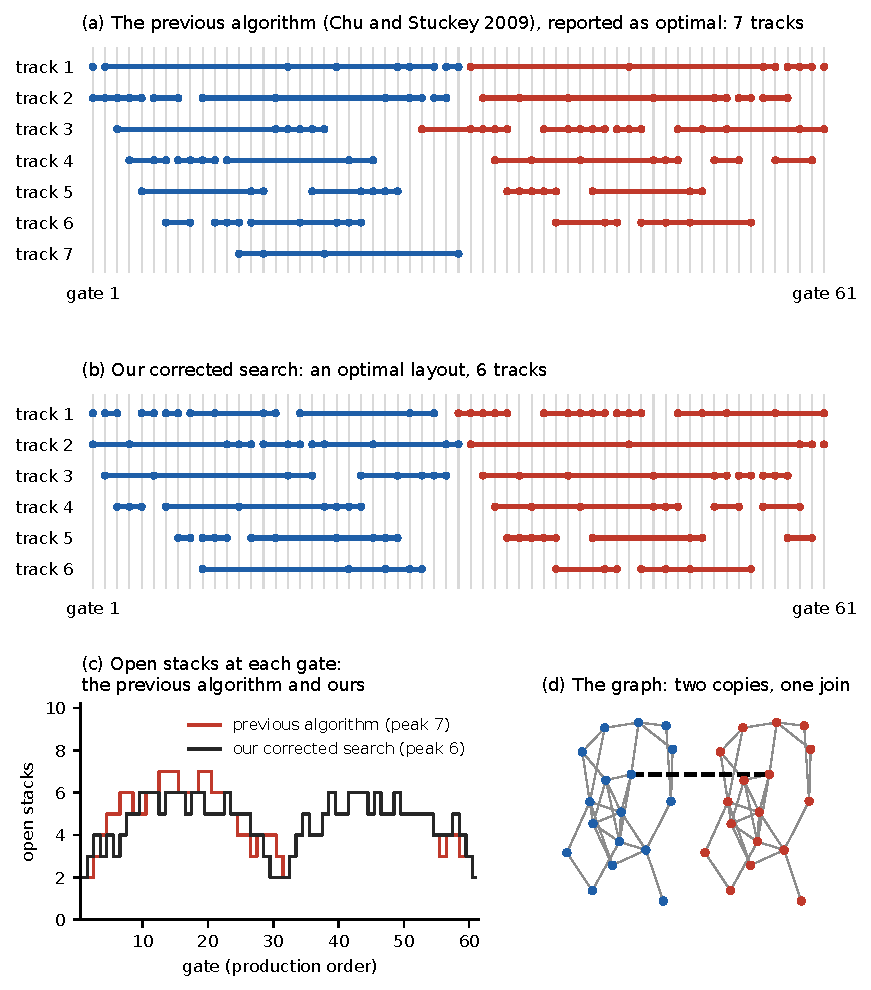
\includegraphics[width=\linewidth]{false_refutation_34.pdf}
\caption{The previous algorithm \citep{ChuStuckey2009} reports a wrong optimum. A 34-customer instance with 61 patterns, drawn as a gate matrix layout of 34 nets on 61 gates. (a) The layout the previous algorithm (our
implementation, better move off) returns and certifies as optimal: 7 tracks. (b) A layout with 6 tracks, found
by our corrected search, which also proves that 5 do not suffice, as do a SAT solver with a DRAT proof checked by drat-trim and Lean (Theorem~\ref{thm:wrong}). (c) The open
stacks at each gate of the two orders: the previous algorithm's order reaches 7 in the
first copy, where the optimal order never exceeds 6.
(d) The instance's graph, two copies of a near-miss joined by one edge.}
\label{fig:wrong}
\end{figure}

\subsection{The rules in pathwidth language}
\label{sec:layouts}

The definite move has an exact counterpart in the pathwidth literature, and
this subsection makes the correspondence precise.
\citet[p.~142]{Kitsunai2016}, stating Tamaki's notion, call an extension $\tau$
of a vertex sequence $\sigma$ \emph{committable} when
$|\partial X'|\ge|\partial V(\tau)|$ for every $X'$ with
$V(\sigma)\subseteq X'\subseteq V(\tau)$. Their Lemma~1 says that if $\sigma$
extends to a feasible permutation, so does $\tau$.

\begin{lemma}\label{lem:endpoint}
For $q\notin S$ and $X=\cl(S\cup\{q\})$: the published premise holds iff
$b(X)\le b(S)$, the commitment condition at the single set $X'=S$; and the
corrected premise holds iff $X$ is a commitment from $S$, the condition at every
$X'$ between them~\leanref{endpoint}.
\end{lemma}

So Theorem~\ref{thm:repaired} is the commitment lemma at the child, and the
published definite move is a commitment whose interior condition was dropped.
In Counterexample~\ref{cex:definite} the endpoint test passes with
$b(X)=3=b(S)$, while the interior set $\{2,3,4\}$ has border
2~\leanref{cexnotcommit}. The published premise is not wasted: by
\citet[Lemma~10, Cor.~2, pp.~148--149]{Kitsunai2016} it guarantees a
commitment to the least-border set between $S$ and $X$, which need not contain
$q$~\leanref{existscommit}. In the counterexample that set is
$\{2,3,4\}$~\leanref{commit234}. Committing there when the matching fails is a
second correction, which gives up no pruning; we have not built it.

A commitment of depth one, $S$ to $S\cup\{q\}$, holds iff
$\open(q,S)\le1$~\leanref{depth1}. The greedy step of
\citet[Lemma~3, p.~49]{CoudertMazauricNisse2014} is exactly that
condition~\leanref{greedy}, and the push rule of
\citet[Rule~1, p.~330]{SuchanVillanger2009} is a case of it. So every published
pathwidth rule of this kind lies in the region $\open\le1$, where the published
definite move is right; \citet[p.~388, Table~2]{KobayashiKomuroTamaki2014}
report depth-one commitments as ``extremely effective''. Chu and Stuckey's
definite move reaches into $\open\ge2$, and that is where it fails. For the
cost of the test, \citet[Cor.~2]{Kitsunai2016} find the least border between
the ends of a given extension by a minimum $s$--$t$ separator;
Theorem~\ref{thm:matching} is that computation for the single target $X$, where
it becomes a bipartite matching.

Table~\ref{tab:known} sums up, and its rows are grouped by what they say. The
published definite and better moves are false. The free move, the memo and
the corrected definite move are known pathwidth results. The subset rule, the corrected
better move and the old move have no counterpart we found, and are proved
here, as is the matching test. The comparison is limited to the pathwidth
papers we have read
\citep{SuchanVillanger2009,Bodlaender2012,CoudertMazauricNisse2014,CoudertMazauricNisse2016,KobayashiKomuroTamaki2014,Kitsunai2016};
``none found'' is not a claim of priority.

\begin{table}[t]
\centering\small
\caption{Two rules of the previous algorithm are false; the free move, the memo and the
corrected definite move are known pathwidth results; the subset rule, the
corrected better move and the old move, like the matching test, are proved here.
Each rule of the customer search against the exact-pathwidth literature.}
\label{tab:known}
\begin{tabularx}{\linewidth}{@{}>{\raggedright}p{3.2cm}>{\raggedright}X>{\raggedright\arraybackslash}p{4.1cm}@{}}
\toprule
Rule & Published counterpart & Status \\
\midrule
definite move, previous algorithm & endpoint case of a commitment (Lemma~\ref{lem:endpoint}) & false (Cex.~\ref{cex:definite}) \\
better move, previous algorithm & none found & false \\
\midrule
free move & full sets \citep{SuchanVillanger2009}; \citet[Prop.~3]{Kitsunai2016} & known \\
definite move, $\open\le1$ & depth-one commitments; greedy step; push rule & known \\
definite move, corrected & commitment lemma \citep[Lemma~1]{Kitsunai2016} & known; matching test (Thm~\ref{thm:matching}) not found \\
memo & subset DP \citep{Bodlaender2012}; prefix and failure tables & known; with the old move, proved here (Thm~\ref{thm:runs}) \\
\midrule
subset rule & none found & proved here \\
better move, corrected & none found & proved here \\
old move & none found & proved here \\
\bottomrule
\end{tabularx}
\end{table}

\paragraph{Prior reports.} We found no earlier report of the error in the 66
works we read in full of the 141 that cite the customer search's papers
(Appendix~\ref{app:prior}). The pathwidth literature has the correct form of
the rule, as a commitment, and none of the pathwidth papers we have read mentions
MOSP.

\subsection{A lower bound from minors}
\label{sec:minor}

The search spends nearly all its effort on one question: whether the value
below the best known one can be refuted. Its floor, contraction degeneracy, is
like every bound built from degrees and cliques a lower bound on treewidth plus
one, so where pathwidth exceeds treewidth no such floor can meet the optimum:
on the Mycielski graph \texttt{myciel6} (95 vertices, pathwidth 38) it is 25.
The pathwidth side of the complex offers a bound with no such ceiling.

\begin{theorem}[minor monotonicity]\label{thm:minor}
Let $G$ be a graph and $uv$ an edge of $G$, and let $G/uv$ be the graph obtained
by merging $v$ into $u$: $u$ becomes adjacent to every neighbour of $u$ or $v$
other than $u$ and $v$, and $v$ is removed. Then $\pw(G/uv)\le\pw(G)$.
Deleting a vertex or an edge never increases pathwidth either. Hence if a
sequence of edge contractions and deletions turns $G$ into $H$, then
$\pw(H)\le\pw(G)$~\leanref{minor}.
\end{theorem}
\begin{proof}
Take a path decomposition $X_1,\dots,X_r$ of $G$ of width $\pw(G)$, and replace
$v$ by $u$ in every bag. No bag grows. Every edge of $G/uv$ either is an edge of
$G$ not touching $v$, which keeps its bag, or joins $u$ to a former neighbour
$x$ of $v$, whose bag held $v$ and $x$ and now holds $u$ and $x$. The bags
holding $u$ were an interval of the path, and so were the bags holding $v$;
since $uv$ is an edge, some bag held both, so the two intervals meet and their
union, the bags now holding $u$, is an interval. So the new bags form a path
decomposition of $G/uv$ of width at most $\pw(G)$. Deleting a vertex or an
edge keeps the decomposition valid with every bag the same or smaller, and the
last claim follows step by step.
\end{proof}

The theorem is the minor-closure of bounded pathwidth, stated for gate matrix
layout by \citet[Lemma~4.2]{FellowsLangston1987}. It gives a certificate of a
lower bound in two parts: a sequence of contractions turning $G$ into a smaller
graph $H$, which anyone can replay, and a refutation of $\pw(H)\le w$, which
then proves $\pw(G)\ge w+1$; on the MOSP graph of an instance, by
Theorem~\ref{thm:mosp}, it proves that every pattern order opens at least
$w+2$ stacks~\leanref{minor}.

\paragraph{The minor step.} Before our corrected search refutes the value
below the best known one, $w$, on the whole graph, it tries to refute $w$ on
minors. It contracts the graph, merging a vertex of least degree into its
neighbour of least degree (or, as a second rule, into the neighbour it shares
fewest neighbours with), to sizes from half the vertices to 85\% of them,
smallest first, and on each minor it runs the same search under a node budget
that triples from one size to the next. A refutation on any minor ends the
descent with the value proved; otherwise the largest width refuted on a minor
raises the lower bound, and the search on the whole graph proceeds as before.
The cost of a refutation grows about tenfold for every five vertices, so the
failed attempts on small minors cost a fraction of the first success, and
climbing from the smallest size costs about as much as knowing the right size
in advance. The idea of solving a contracted graph exactly for a lower bound
is used for treewidth \citep{BodlaenderWolleKoster2006,BodlaenderKoster2011};
for pathwidth it is not capped by treewidth, which is where the rest of the
floor stops. Section~\ref{sec:pwsolver} reports what it settles.

% Section 5, computational results and the dataset (loop0009 item 06; was old
% Sections 4.6-4.7). Sources: paper1/solver_fix.md (cost, re-certification, the
% split and its addendum), paper1/certificates.md (proof object),
% paper1/dataset.md (the dataset, its checker and its price). Tables from
% tables/ (make_tables.py). Setup: lscpu and free on the machine that ran
% everything, read 2026-10-06; compiler flags from satisfiability/native.py.
\section{Computational results and a dataset}
\label{sec:results}

Section~\ref{sec:search} proved our corrected search sound. This section asks
five practical questions about it and answers each with a measurement. What
does our correction cost? At most 2\% more search nodes on each group of benchmarks we measured. Do the published
benchmark optima survive? All 115 that rested on the previous algorithm
\citep{ChuStuckey2009} were proved again, and none changed. How good a
pathwidth solver is it? On every benchmark set with published exact counts it proves as many or more graphs than the published branch and bound of \citet{CoudertMazauricNisse2016}, and it is faster on each of the fourteen graphs whose times they publish. Can a reader check a refutation without
trusting our code? Yes, up to about 75 customers, through a certificate and an
independent checker. Finally, what does it make possible? A dataset of 17,714
graphs from twenty benchmark collections. For 16,634 of them the pathwidth is
certified, and that gives the exact value of every problem in the exact core.

\subsection{Experimental setup}
\label{sec:setup}

\paragraph{Machine and code.} Every run in this section used one
machine, an AMD Ryzen~9 9950X (16 cores, 32 hardware threads) with 128\,GB of
memory under Ubuntu Linux. Both searches, the open-stacks customer search and
its port to graphs, are written in C, compiled with gcc 15.2 using the
flags \texttt{-O3} and \texttt{-march=native}, and driven from Python~3.12. A Python implementation of the
same rules serves as a reference for cross-checks and emits the certificates
of Section~\ref{sec:certs}. Our corrected tests are the default in every
implementation; the tests of the previous algorithm remain available as an option. The C
implementation handles components of at most 1,024 vertices; 154 classes of
the dataset of Section~\ref{sec:dataset} are larger.

\paragraph{Runs.} The basic job asks one question: is the optimum of this
instance at most $k$? A \emph{worker} is one single-threaded process that
answers such questions, one at a time. A \emph{node} is one state visited by
the search, the unit in which we report effort. Up to 32 workers ran at
once on the machine, so wall-clock times carry load noise. We therefore
compare node counts and report time only in \emph{core-hours}, the hours of one core summed over workers (32 workers for one hour make 32 core-hours). A \emph{pair} runs
the same question twice in the same worker, once under the previous algorithm
and once under our corrected rules, alternating which goes first. A
\emph{descent} solves a whole graph: it lowers $k$ from an upper bound until a
refutation proves the last value optimal. Each table states its time or node
budget.

\paragraph{Configurations.} The open-stacks runs use two configurations of the
rules of Section~\ref{sec:search}, which differ only in the better move. The
\emph{base} configuration leaves it off. The configuration \emph{with better
move} switches it on for instances whose customers need at most five patterns on
average. This is the setting under which our implementation of the previous algorithm certified the benchmark values it proved.

\paragraph{Instances.} The \emph{MOSP corpus} is the 6,376 instance files of
four public open-stacks collections, one of which is distributed twice. They
are the 2005 Constraint Modelling Challenge \citep{SmithGent2005}, with a
second copy of 46 of its files under other names, the random
instances of \citet{ChuStuckey2009} (30 to 125 customers), those of
\citet{FaggioliBentivoglio1998}, and the 24 industrial instances of the SCOOP project, real instances from two sawmilling companies \citep{Frinhani2018}. They
are the first rows of Table~\ref{tab:dataset}. A Chu--Stuckey name such as
\texttt{Random-125-125-2-4\_0} gives the number of customers, the number of
patterns, the generator's density class (roughly, the number of customers per pattern) and the instance number. The graph benchmarks are those of Table~\ref{tab:dataset}.

\paragraph{Provenance.} Every stored value comes with a witness, an order that
attains it, and one of three provenances:
\begin{itemize}
\item \emph{certified by search}: a search proved that no order does better,
  by refuting the value minus one;
\item \emph{certified by bound}: a lower bound equals the witness's value, so
  no search was needed;
\item \emph{upper bound only}: the witness is all there is, and optimality is
  not proved.
\end{itemize}
All 6,376 corpus values are certified (as of 12 October 2026; the last two were
certified by the split search of Section~\ref{sec:practice}).

\subsection{The cost of our correction, and the benchmark values}
\label{sec:practice}

Our corrected search adds one matching test to the definite move and to the
better move (Section~\ref{sec:definite}). A candidate that fails the matching
is passed over, so the corrected tree can only differ where the matching fails.
Table~\ref{tab:cost} shows how rarely that matters.

\begin{table}[t]
\centering\small
\caption{Our correction never changed an answer and costs at most 2\% more
nodes in total. Each pair runs the same question under the previous algorithm and under the
corrected rules in one worker. Totals are over the pairs that finished under
both rules; a pair stopped by its budget says nothing about cost.
\emph{Vertices}: customers in the open-stacks rows (the vertices of $G_M$).
\emph{Largest pair ratio}: the largest ratio of corrected to previous nodes
over single pairs. Open-stacks pairs refute the optimum minus one, at 600\,s per
call at 50--100 customers and $2\times10^8$ nodes at 125. The graph pairs run
whole descents on VSPLIB, the colouring and named graphs, and a sample of 500
Rome graphs.}
\label{tab:cost}
\resizebox{\linewidth}{!}{% Generated by python -m paper1.latex.make_tables. Source: paper1/data/solver_fix_cost_{mosp40,cs,cs125,pw}.csv.
% Do not edit by hand.
\begin{tabular}{@{}llrrrrr@{}}
\toprule
Instances & Vertices & Pairs finished & Nodes, previous & Nodes, repaired & Total ratio & Largest pair ratio \\
\midrule
\multicolumn{7}{@{}l}{\emph{Open stacks: one refutation of the optimum minus one per pair}} \\
\quad MOSP corpus, base & 9--40 & 6,135 of 6,135 & 228,147 & 228,154 & 1.00003 & 1.009 \\
\quad MOSP corpus, with better move & 9--40 & 6,135 of 6,135 & 202,962 & 202,971 & 1.00004 & 1.040 \\
\quad Chu \& Stuckey, with better move & 50--100 & 118 of 125 & 1,358,096,671 & 1,362,205,210 & 1.00303 & 1.013 \\
\quad Chu \& Stuckey, cap $2\times10^8$ nodes & 125 & 11 of 23 & 90,969,508 & 90,961,419 & 0.99991 & 1.000 \\
\addlinespace
\multicolumn{7}{@{}l}{\emph{Graph pathwidth: one whole descent per pair, 120\,s each}} \\
\quad VSPLIB, colouring, named, 500 Rome & 4--2{,}916 & 731 of 880 & 2,977,849,807 & 3,038,670,717 & 1.020 & -- \\
\bottomrule
\end{tabular}
}
\end{table}

In every row of Table~\ref{tab:cost} our corrected search and the previous algorithm gave
the same answer, and the total node counts differ by at most 2\%. Single
open-stacks pairs differ by at most 4\%. The time per node also rises, by about 2\% in the C
implementation, measured on six hard instances at 75 to 125 customers. The
published test passes and the matching then fails on only 0.07--0.27\% of
definite-move candidates, a rate that rises with size.

\paragraph{The benchmark values survive.} None of the 115 values changed under
our corrected rules. Of the 6,374 values certified before this work, 6,259 do
not depend on the customer search at all. Each was proved in one of four ways:
\begin{itemize}
\item by an exhaustive computation over all subsets of customers (up to 15
  customers);
\item by a refutation from a SAT (Boolean satisfiability) solver whose proof an
  independent checker accepted, in DRAT, the standard proof format for SAT
  solvers;
\item by an earlier SAT search;
\item or by a lower bound equal to the value.
\end{itemize}
The other 115 rested on the customer search
of the previous algorithm. Our corrected search refuted the value minus one on
all 115, so all 115 values stand. They are 115 benchmark entries on 113
distinct graphs: SP3 and SP4 are each stored twice.

The seven hardest are 125-customer Chu--Stuckey instances at density classes 2
and 4. They are too large for one worker, so their search was split:
the top levels of the tree are expanded into independent subtrees, each
refuted on its own worker, and the value is refuted when every subtree is. The
split is proved sound~\leanref{split}. All seven were refuted at 18 to 369
core-hours each, 1,112.6 in total (Table~\ref{tab:split},
Appendix~\ref{app:split}).

\paragraph{Two values never certified before.} The corpus also held two values that
no method had certified: 25 for \texttt{Random-125-125-2-2\_0} and 21 for
\texttt{Random-125-125-2-3\_0}. The same split refutes the value minus one on
each. On 9 October 2026 it refuted 20 for \texttt{Random-125-125-2-3\_0}, after
9,665 subtrees, $4.25\times10^{12}$ nodes and 1,128 core-hours, which
certifies 21 as its optimum. On 12 October 2026 it refuted 24 for
\texttt{Random-125-125-2-2\_0}, after 17,001 subtrees,
$7.38\times10^{12}$ nodes and 2,231 core-hours (Table~\ref{tab:split}), which
certifies 25; it is the largest refutation in this paper. With it, every value
of the MOSP corpus is certified. The minor step of Section~\ref{sec:minor}
reaches two of these values in seconds: a 69-customer minor of \texttt{Random-125-125-2-3\_0} refutes 20 in 666,153
nodes, under a second of search, against
1,128 core-hours on the full instance, and an 87-customer minor of
\texttt{Random-125-125-2-1\_0} refutes 23 in 30\,s with a larger budget, against 366.5 core-hours
(Table~\ref{tab:split}). It does not reach
\texttt{Random-125-125-2-2\_0}: every minor of up to 95 customers that we tried admits 24. The minor bound
also equals the optimum on \texttt{Random-125-125-6-1\_0} (81) and SP4 (53),
which the search refutes on the full instance within a minute.

\subsection{Our corrected search as a pathwidth solver}
\label{sec:pwsolver}

Ported to graphs, our corrected search is an exact pathwidth solver. Table~\ref{tab:graphs} gives what it proves on the 11,915 benchmark graphs it was run on, counted as files, beside the run of the previous
algorithm under the same caps and the published counts of
\citet{CoudertMazauricNisse2016}. Where both runs prove a graph, the widths
agree on every one. The 24 Rome graphs proved only by the corrected run, and the
13 proved only by the previous one, sit near the 600\,s cap. The comparison with
\citet{CoudertMazauricNisse2016} is with published numbers obtained on other
hardware, not a head-to-head run. On the fourteen graph-colouring benchmarks of TreewidthLIB whose times
\citet[Table~4]{CoudertMazauricNisse2016} report, our search proves the same
pathwidth and is faster on every one: by 150 to 1,800 times on \texttt{david},
\texttt{miles750} and \texttt{mulsol.i.5}, by 70 to 80 times on
\texttt{miles1000} and \texttt{zeroin.i.1}, and by 1.4 to 10 times on the
other nine, where a hardware difference could account for the margin. It also
proves \texttt{queen11\_11} (pathwidth 87) in 37\,s and \texttt{queen12\_12}
(103) in 391\,s, beyond their table, and \texttt{fpsol2.i.1} (496 vertices,
pathwidth 67) in 5.7\,s, against 323\,s for
\citet{KobayashiKomuroTamaki2014}. Without the minor step, one graph goes the other way: the Mycielski graph
$M_7$ (\texttt{myciel6}, 95 vertices, pathwidth 38), which their tuned branch
and bound proves in about ten minutes, while the full refutation of 37 by our
search does not finish in hours, its floor being 25. Mycielski graphs are
built to have no triangles and yet to need many colours, so their largest
cliques are single edges and their degrees are uneven: the degree and clique
bounds that make up our floor see almost nothing. Their pathwidth also
exceeds their treewidth (38 against 35 here), so no bound on treewidth can
reach it.

\paragraph{With the minor step.} The minor step of Section~\ref{sec:minor}
changes this. A 58-vertex minor of \texttt{myciel6} already has pathwidth 38,
and the step proves $\pw=38$ in 0.2\,s. On \texttt{myciel7} (191 vertices),
which \citet{CoudertMazauricNisse2016} leave open with $\pw\le72$, a
110-vertex minor proves $\pw\ge71$; the best published lower bound we found is
the treewidth bound 52 of \citet{BodlaenderWolleKoster2006}, so $\pw$ is 71 or
72. Of the 340 Rome graphs left open by the 600\,s run of
Table~\ref{tab:graphs}, the step proves 271 within 60\,s each (median 0.5\,s),
and 292 with a larger budget; we refuted the other 48 without a time limit,
the longest in 25.4 hours, so the pathwidth of every one of the 11,534 Rome
graphs is now proved;
the Harwell--Boeing count rises from 39 to 43, and the colouring benchmarks
gain \texttt{anna} and \texttt{myciel6}. The VSPLIB grids need no search: each
is an $n\times n$ grid, whose pathwidth is $n$ by
\citet[Theorem~4.1]{EllisWarren2008}, and a row-by-row layout of width $n$ attains it, so all 50 are settled where
search alone proved 9. We machine-checked the theorem~\leanref{grid}, by a
direct argument on vertex separation: at the first prefix of any layout that
completes a row or a column, the boundary meets every column or every row.
That each VSPLIB grid is an $n\times n$ grid is checked by an isomorphism
test, not in Lean. On graphs proved both with and without
the step, it lowers the total node count by 55 to 99\% on Rome, the VSPLIB grids,
Harwell--Boeing and the colouring graphs, adds 1\% on the named graphs and
20\% on the VSPLIB trees (about 1.5\,s a tree), and costs 4\% of the time on
a sample of 120 MOSP corpus instances. The minor bounds for \texttt{myciel6},
\texttt{myciel7} and the four MOSP instances below were also refuted by a
separate exact search that uses no dominance rule and writes out every refuted
set, which an independent checker verifies. Their branch and bound is openly available in SageMath, and a
head-to-head run on one machine is the comparison that would settle which solver is stronger; we have not yet made it.

\begin{table}[t]
\centering\small
\caption{Our corrected search as a pathwidth solver. Graphs whose pathwidth it
proves, under our corrected rules and under the previous algorithm with the same
caps (Rome: 10, 120 and 600\,s in stages), without the minor step of
Section~\ref{sec:minor}, and the published counts of
\citet{CoudertMazauricNisse2016} under a 10-minute cap. \emph{Width differs}:
graphs proved by both runs with different widths. $^{a}$All 50 VSPLIB grids:
each is an $n\times n$ grid, checked by isomorphism, so its pathwidth is $n$ by
\citet[Theorem~4.1]{EllisWarren2008}; the 41 that search did not prove carry a
witness layout of width $n$.}
\label{tab:graphs}
\resizebox{\linewidth}{!}{% Written by hand from paper1/solver_fix.md, item 08, "Table 1: proved widths,
% corrected against old, same caps", and from Coudert, Mazauric & Nisse (2016)
% as recorded in pathwidth_solver/bench/reference.py.
\begin{tabular}{@{}lrrrrrl@{}}
\toprule
Set & Vertices & Graphs & Proved, corrected & Proved, previous & Width differs & \citet{CoudertMazauricNisse2016} \\
\midrule
Rome & 10--110 & 11,534 & 11,194 & 11,183 & 0 & 95.6\% (ours 97.1\%) \\
VSPLIB trees & 22--202 & 50 & 50 & 50 & 0 & 30 \\
VSPLIB Harwell--Boeing & 24--960 & 73 & 39 & 39 & 0 & 26 \\
VSPLIB grids & 25--2{,}916 & 50 & 9 & 9 & 0 & 9 (sides 5--13) \\
TreewidthLIB colouring & 5--864 & 58 & 31 & 31 & 0 & all 14 held agree \\
freetdi named & 4--3{,}282 & 150 & 125 & 125 & 0 & -- \\
\midrule
All & & 11,915 & 11,448 & 11,437 & 0 & \\
\bottomrule
\end{tabular}
}
\end{table}

\paragraph{What a proof costs.} Figure~\ref{fig:cost} plots the search nodes
of every width our search has proved, on 8,510 graphs, against the number of
vertices $n$ and against $n$ times the width $w$. On the Rome graphs, sparse
graph-drawing instances, the cost follows one law,
\[
  \log_{10}(\text{nodes}) \approx 1.75 + 0.00705\, n w ,
\]
with $r^2=0.96$ and a typical graph within a factor of 2.3 of it: each further
100 in $nw$ multiplies the work about fivefold. Size alone explains less
($r^2=0.85$), and so does width alone (0.89); the states of the search are
vertex sets whose boundary has at most $w$ vertices, and their number grows
with both. The 48 hardest Rome graphs, which we refuted without a time limit
(the longest in 25.4 hours), lie above the line, so the law ranks
graphs by hardness but understates the extreme tail. Graphs that the 600\,s
runs did not finish are absent, so the top of the curve is a lower envelope.
The structured sets do not follow the Rome law: Harwell--Boeing graphs of up
to 960 vertices, the colouring and named graphs and the dataset's open classes
are proved with orders of magnitude fewer nodes than it predicts, mostly
because a lower bound, often from a minor, meets the width early. Time tracks
nodes closely ($r^2=0.98$), which is why we report nodes.

\begin{figure}[tbp]
\centering
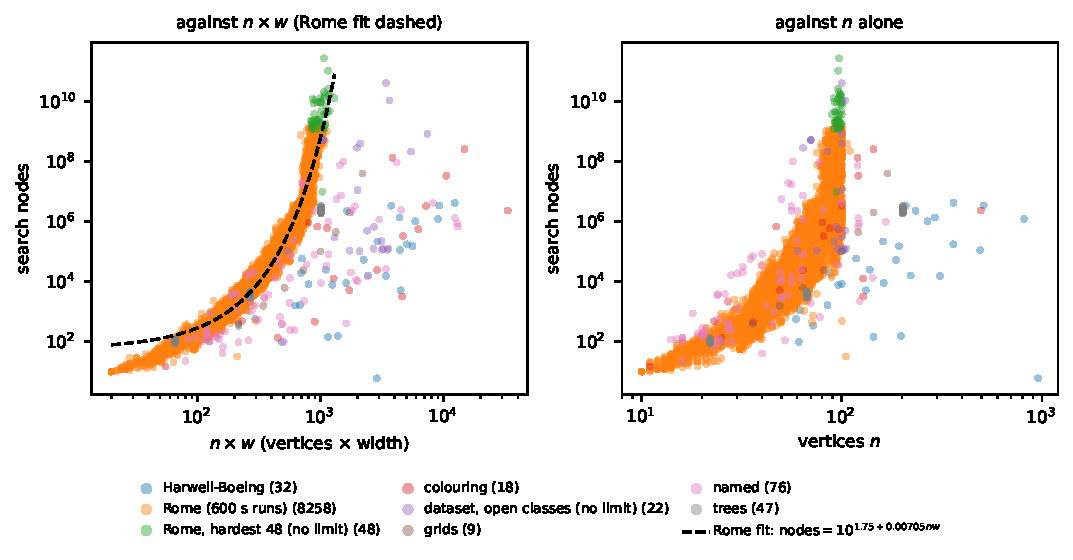
\includegraphics[width=\linewidth]{solve_times.pdf}
\caption{The cost of proving a pathwidth. Search nodes for every width our
search has proved (8,510 graphs, both axes logarithmic), against $n$ times the
width (left) and against $n$ alone (right). The dashed line is the fit on the
Rome graphs, $\text{nodes}=10^{1.75+0.00705\,nw}$. The structured benchmark
sets fall far below it, and size alone gives no single law.}
\label{fig:cost}
\end{figure}

\subsection{A checkable proof of a refutation}
\label{sec:certs}

A refutation by the search is a claim about a tree of up to $10^{12}$ nodes,
and Theorem~\ref{thm:main} proves the rules sound, not the code that runs
them. So the search emits a \emph{certificate}: the tree it explored, every
pruning step with its rule and its witness, and for each definite and better
step the matching of Theorem~\ref{thm:matching}. An independent checker, which
shares no code with the search, reads the instance matrix and the certificate.
At every node it checks that
\begin{itemize}
\item the premise of every pruning step holds, recomputed from the matrix;
\item every matching is valid: distinct customers, distinct stacks, each stack
  newly opened by its customer, and at least $\open-1$ edges;
\item every candidate within the bound is either a child or covered by a
  pruning step, and every chain of covers ends at a child or an old move,
  with no cycle;
\end{itemize}
and it replays the tree from the root. Each accepted step is a Lean theorem.
That an acyclic covering by such steps is sound is a short paper argument, not
yet a formal proof.

\begin{table}[t]
\centering\small
\caption{Every certificate the search emitted verifies, none is rejected, and
checking takes milliseconds. Certificates for our corrected rules, configuration
with better move, refuting the optimum minus one on the certified MOSP corpus
at 9--75 customers, with 60\,s to emit each. \emph{Not emitted}: the emitter
did not finish in time. Size is the compressed certificate; check time is the
independent checker's.}
\label{tab:certs}
\resizebox{\linewidth}{!}{% Generated by python -m paper1.latex.make_tables. Source: paper1/data/certificates/corrected.csv.
% Do not edit by hand.
\begin{tabular}{@{}lrrrrrr@{}}
\toprule
Customers & Instances & Verified & Rejected & Not emitted & Median size (bytes, gzip) & Median check (ms) \\
\midrule
9--10 & 1,614 & 1,614 & 0 & 0 & 332 & 0.04 \\
11--20 & 2,508 & 2,508 & 0 & 0 & 356 & 0.08 \\
21--30 & 1,816 & 1,816 & 0 & 0 & 414 & 0.24 \\
31--40 & 197 & 197 & 0 & 0 & 650 & 1.27 \\
41--50 & 120 & 120 & 0 & 0 & 12,045 & 33.24 \\
51--60 & 1 & 1 & 0 & 0 & 126,508 & 278.86 \\
61--75 & 30 & 19 & 0 & 11 & 26,516 & 143.70 \\
\bottomrule
\end{tabular}
% total csearch: 6275 of 6286 verified, 0 rejected, 35.47 MB gz, 147.4 s, 3353245 nodes
% total default: 6276 of 6286 verified, 0 rejected, 54.77 MB gz, 242.3 s, 5361282 nodes
}
\end{table}

Table~\ref{tab:certs} gives the results. Every refutation emitted within its
budget verifies, 6,275 of 6,286, and none is rejected. All 35.5\,MB of
certificates check in 147\,s. The base configuration gives the same picture:
6,276 of 6,286 verify and none is rejected. The checker also catches the error
of Section~\ref{sec:definite}. On the graph of
Counterexample~\ref{cex:definite}, rooted at $\{2\}$, the previous algorithm emits
a complete tree that claims there is no solution. A checker of the published
premises accepts it. Ours rejects it, even with a largest matching attached,
because the matching has one edge where two are needed. At 125 customers the
trees are too large to ship as certificates.

\subsection{A dataset with certified pathwidth}
\label{sec:dataset}

Section~\ref{sec:equiv} showed that one certified pathwidth $w$ answers every
problem in the exact core. Pathwidth, vertex separation and the vertex
separator game take the value $w$, and MOSP, gate matrix layout (which
multiple folding equals), one-dimensional logic, interval thickness,
narrowness, node search, progressive pebbling, the vertex search of
\citet{BRST1991} and the maximum wavefront take $w+1$: twelve problems in all, counting multiple folding with gate matrix layout. We therefore built one dataset from every benchmark collection of
those problems that we could obtain, including the MOSP corpus.

The unit of the dataset is the \emph{isomorphism class}: the set of instances
whose graphs are the same up to renaming the vertices. For a matrix instance
the graph is its MOSP graph. Two instances in one class have the same value
under every problem, so the dataset holds one record per class, with its
members and the renaming that maps each onto the record's graph. Classes were
found with nauty, a standard tool that computes a canonical form for each
graph. Each record carries the graph, the width $w$, its provenance, and a
witness layout of exactly that width. A record certified by bound also carries
a \emph{minor certificate}: a list of vertex deletions and edge contractions
after which every vertex has degree at least $w$. Any checker can replay it,
and it proves the pathwidth is at least $w$. A record certified on a minor
carries, when it is stored, the sequence of edge contractions that gives
the minor on which our search refuted width $w-1$, which proves $\pw\ge w$ by
Theorem~\ref{thm:minor}. A record certified by theorem names the theorem and
its Lean proof; so far these are the VSPLIB grids, whose pathwidth is given by
the grid theorem~\leanref{grid}.

\begin{table}[t]
\centering\small
\caption{Twenty collections, 21,754 instance files, reduce to 17,714
isomorphism classes, and 16,634 of them have a certified pathwidth with a
witness layout. Largely open: PACE, the VSPLIB Harwell--Boeing graphs, and the
MOSP sets of de Carvalho and Soma and of Frinhani et al. \emph{Classes}: isomorphism classes within the
collection (78 graphs above 5,000 vertices are compared by file content only).
\emph{Counted here}: classes whose first member, in the order of the table,
is in this collection, so the column sums to the dataset's class count. The
next six columns split those classes by provenance: certified by search on
the graph, by search on a contracted minor (Theorem~\ref{thm:minor}), by a
lower bound, or by a theorem; or an upper bound only. \emph{No witnessed
value}: no layout is stored yet; this includes one Rome class whose pathwidth
is certified but which has no stored layout of that width. $^{a}$The same 46 files distributed a second
time under other names; every class is counted under its first copy.}
\label{tab:dataset}
\resizebox{\linewidth}{!}{% Generated by python -m paper1.latex.make_tables. Source: paper1/data/dataset/{index,classes}.csv.gz.
% Do not edit by hand.
\begin{tabular}{@{}lrrrrrrrrr@{}}
\toprule
 & & & & \multicolumn{4}{c}{Certified} & & \\
\cmidrule(lr){5-8}
Collection & Files & Classes & Counted here & by search & on a minor & by bound & by theorem & Upper bound only & No witnessed value \\
\midrule
MOSP: Challenge 2005 & 5,806 & 3,169 & 3,169 & 3,168 & 0 & 1 & 0 & 0 & 0 \\
MOSP: Challenge 2005 (second copy)$^{a}$ & 46 & 46 & 0 & 0 & 0 & 0 & 0 & 0 & 0 \\
MOSP: Chu \& Stuckey & 200 & 200 & 200 & 200 & 0 & 0 & 0 & 0 & 0 \\
MOSP: Faggioli \& Bentivoglio & 300 & 287 & 274 & 274 & 0 & 0 & 0 & 0 & 0 \\
MOSP: SCOOP & 24 & 24 & 24 & 24 & 0 & 0 & 0 & 0 & 0 \\
VLSI gate matrix circuits & 11 & 11 & 11 & 5 & 0 & 5 & 0 & 1 & 0 \\
VSPLIB trees & 50 & 28 & 28 & 28 & 0 & 0 & 0 & 0 & 0 \\
VSPLIB grids & 50 & 50 & 50 & 9 & 0 & 0 & 41 & 0 & 0 \\
VSPLIB Harwell--Boeing & 73 & 72 & 72 & 32 & 5 & 7 & 0 & 28 & 0 \\
Small (Marti et al. 2008) & 84 & 84 & 84 & 32 & 0 & 52 & 0 & 0 & 0 \\
Rome graphs & 11,534 & 11,199 & 11,199 & 8,166 & 286 & 2,746 & 0 & 0 & 1 \\
TreewidthLIB colouring & 58 & 58 & 58 & 18 & 2 & 13 & 0 & 25 & 0 \\
freetdi named graphs & 150 & 146 & 143 & 103 & 1 & 22 & 0 & 16 & 1 \\
freetdi control-flow graphs & 1,817 & 1,070 & 1,064 & 398 & 2 & 661 & 0 & 2 & 1 \\
MOSP: Frinhani et al. 2018, large & 610 & 610 & 610 & 0 & 0 & 0 & 0 & 0 & 610 \\
PACE 2016 & 291 & 288 & 112 & 38 & 13 & 18 & 0 & 37 & 6 \\
PACE 2017 exact & 200 & 199 & 193 & 61 & 61 & 7 & 0 & 54 & 10 \\
PACE 2017 heuristic & 200 & 197 & 173 & 11 & 5 & 3 & 0 & 40 & 114 \\
PACE 2017 bonus & 100 & 100 & 100 & 24 & 54 & 0 & 0 & 22 & 0 \\
MOSP: Carvalho \& Soma 2015 & 150 & 150 & 150 & 38 & 0 & 0 & 0 & 112 & 0 \\
\midrule
All & 21,754 &  & 17,714 & 12,629 & 429 & 3,535 & 41 & 337 & 743 \\
\bottomrule
\end{tabular}
}
\end{table}

Table~\ref{tab:dataset} gives the counts. The collections are the MOSP
collections
\citep{SmithGent2005,FaggioliBentivoglio1998,ChuStuckey2009,CarvalhoSoma2015,Frinhani2018},
eleven VLSI gate matrix circuits \citep{OliveiraLorena2002}, the VSPLIB sets
\citep{Duarte2012} and the Small graphs \citep{MartiCamposPinana2008}, the Rome
graphs \citep{DiBattista1997}, and treewidth collections used as pathwidth
benchmarks \citep{TreewidthLIB,freetdi,PACE2016,PACE2017}. Of the 17,714
classes, 16,634 carry a certified pathwidth with a witness layout and 337 a witnessed upper bound, and 743 have no witnessed value yet, one of them with a certified pathwidth. The 610 large instances of \citet{Frinhani2018}, with
400 to 1,000 customers, are included so that the dataset covers every
published MOSP collection we have. None of them has a value yet, because an
exact search at that size is out of reach.

An independent checker, sharing no code with the solvers, verifies the
dataset. It re-reads all 20,984 member files with its own readers, maps each
onto its record's graph by its renaming, recomputes the width of every witness
layout, replays every minor certificate and every stored contraction sequence
(424 of the 429 records certified on a minor), and recognises each grid
certified by theorem from its edges alone. It reports no failure on the
16,971 records, the 16,634 certified classes and the 337 with an upper bound. A value certified by search cannot be checked from its record,
and neither can the refutation on a minor;
both rest on our corrected search, and for instances within reach of the emitter
the certificate of Section~\ref{sec:certs} is how a third party can check it.

\paragraph{Agreement with published values.} All 84 Small graphs agree with
the pathwidths of \citet[Tables~4--5]{Mallach2018}. Ten of the eleven VLSI
circuits are certified at their published best-known track counts
\citep[Table~I]{OliveiraLorena2002}; the eleventh, W4 with 202 nets, is open
at 28 against 27.

\paragraph{A caution about MOSP files.} A MOSP file can be read with rows as
customers or with rows as patterns, and the two readings give different
graphs. The same public repository ships the
\citet{CarvalhoSoma2015} instances as customers by patterns and the
\citet{ChuStuckey2009} instances beside them as patterns by customers. Only
published densities and values tell them apart. Read the wrong way round, an
instance certifies at a different value.

% Section 6. Written by loop0009 item 09 (review section 3, "Section 5,
% Closing"). Every claim is from the body: Section 2 summary (rows), Section 3
% (communities), Sections 4.3-4.5 (rules), Section 5 (cost, values, certificates,
% dataset). The in-flight status is `python -m paper1.solver_fix_split
% --summary`, checked 2026-10-06. The price of the open classes is
% paper1/dataset.md section 6 (moved here from Section 5.4 by item 06).
\section{Conclusion}
\label{sec:closing}

We asked which equalities of the Linhares--Yanasse table are true, and what
follows when results, algorithms and benchmarks are moved between its twelve
problems through pathwidth. Eight rows are exact, counting the pathwidth row
itself: each of those eight problems is pathwidth, or pathwidth plus one, on
every input. Two rows, split bandwidth and edge search, are bands
one and two wide, and two, PLA folding and edge separation, are false as stated,
although a variant of each is exact (Table~\ref{tab:master}). This is the
sense in which the family is a pathwidth complex: its exact members are one
quantity, and the literature names that quantity pathwidth. Moving between
the problems paid twice. Read as a pathwidth algorithm, the best exact
open-stacks search turned out to rest on two false dominance theorems; our
corrected definite move was also found by Tamaki as a lemma \citep[Lemma~1]{Kitsunai2016}, and with it and our corrected better
move the search is sound. And one
certified pathwidth answers every problem in the exact core at once, which is
what made a single dataset for twelve problems possible, three of them
problems the table did not list, one from a fourth discipline, numerical
linear algebra.

\paragraph{What transfers, and what does not.} Within the exact core, anything
proved or computed for one problem holds for the others with the offset of
Table~\ref{tab:master}: an algorithm, a lower bound, a benchmark value. Across
a band only an approximation transfers. Split bandwidth and edge search stay
within one of the number of open stacks, as the table's literal reading says,
but not at a fixed offset, so an exact value of one does not give an exact
value of the other. Across a false row nothing transfers. Simple PLA folding
can need arbitrarily more tracks than the pathwidth suggests, and cutwidth is
not within a constant of pathwidth on stars. Section~\ref{sec:names} showed why
these distinctions went unchecked for two decades: the communities rarely read
one another, and most of what is known about the family is published under
``pathwidth''.

\paragraph{What the search teaches about dominance rules.} The two false
theorems were published in 2009 and restated in later work, and the
implementations that use them reported no failure. On every benchmark, and in
every run of our checks where the previous algorithm \citep{ChuStuckey2009} lost the last solution at a
node, another branch found a solution (Section~\ref{sec:theorem}). It took a
search built for the purpose to find a whole instance with a wrong optimum,
34 customers and one stack too many (Figure~\ref{fig:wrong}), in our
implementation of the previous algorithm with the better move off; the optimum
of 6 is confirmed by a SAT solver with a DRAT proof checked by drat-trim. So the absence of
wrong answers on benchmarks was never evidence that the rules were sound. Three things in this paper bear on that. Reading the rules in pathwidth language put the correct rule, the
commitment lemma, beside the published one. Proving each rule on its own was
not enough: the order in which the rules run matters, because a cycle of true
links can still lose a node (Section~\ref{sec:theorem}). And a certificate
whose checker recomputes every premise rejects the false refutation that a
checker of the published premises accepts (Section~\ref{sec:certs}). Our correction
is cheap: one bipartite matching per candidate and at most 2\% more nodes per
benchmark set. Our corrected search re-proved all 115 benchmark optima that
rested on the previous algorithm, and changed none.

\paragraph{What a reader can do differently.} Cite our table as corrected here,
Table~\ref{tab:master}, rather than the 2002 one. Look for results on MOSP and
gate matrix layout under ``pathwidth''. Use our corrected search as an exact
pathwidth solver. On every benchmark set with published exact pathwidth counts
it proves as many or more graphs than the published branch and bound of
\citet{CoudertMazauricNisse2016} (Table~\ref{tab:graphs}). We believe it is
currently the strongest exact pathwidth solver openly available, and it is open
source. And in any implementation of the rules
of \citet{ChuStuckey2009}, including the code behind the optima of
\citet{Frinhani2018} that \citet{MartinYanassePinto2022} reuse
(Appendix~\ref{app:prior}), replace the definite and better moves of the previous algorithm
with the matching test. The values those implementations report are not known
to be wrong, but their refutations are not proved.

\paragraph{Limits.} Six limits remain.
\begin{itemize}
\item The Lean model of the search and the C and Python code that run it are
  linked by testing and by certificates, not by proof
  (Section~\ref{sec:theorem}).
\item That an acyclic covering by checked steps is sound, which is the
  certificate checker's acceptance condition, is a paper argument
  (Section~\ref{sec:certs}).
\item LaPaugh's equality $\es=\pes$ is stated and not formalised. No row
  needs it (Section~\ref{sec:true}).
\item One reference of the table, \citet{LY2002ref5}, is not held. Its row,
  interval thickness, is proved from two other
  references of the table
  (Section~\ref{sec:true}).
\item The comparisons of the graph solver are with published numbers obtained
  on other hardware, not head-to-head runs, and only against
  \citet{CoudertMazauricNisse2016}. On one graph they report, the Mycielski
  graph $M_7$ (95 vertices, pathwidth 38), their tuned branch and bound proves
  the pathwidth in about ten minutes, and our search did not within 25 minutes.
\item The census of names covers the twelve names of the table; the three
  members we add, and the wider treewidth and pebbling literatures, are not
  counted (Section~\ref{sec:names}).
\end{itemize}

\paragraph{Open problems.} One value of the MOSP corpus,
\path{Random-125-125-2-2_0}, has never been certified. As of 9 October 2026 the
split search is still refuting the value minus one and has found no order of
the smaller value; the other value that was open, \path{Random-125-125-2-3_0},
was certified on 9 October (Section~\ref{sec:practice}). Of the 17,714 classes of the dataset, 1,627 have
no certified pathwidth. One more budget step for every open class within the
size our implementation handles costs at most 500 core-hours, but on the Rome graphs each such step has closed only about
40\% of what it attempted, so the graph sets will not close by budget alone.
The 610 MOSP instances with 400 to 1,000 customers, and the 154 classes above
the implementation's limit of 1,024 vertices per component
(Section~\ref{sec:setup}), are beyond an exact search. Beyond budgets, a class is certified without search
only when a lower bound meets its witness (Section~\ref{sec:dataset}). The
open classes are therefore also a test set for stronger lower bounds on
pathwidth.

% The data, code and proofs statement (loop0009 item 01). It replaces the
% title-page footnote and every file path and `python -m` command that the
% body used to carry. Those commands, kept here for later items and recorded
% in the paper1/*.md documents that are the sources of record:
%   Section 3 figures and numbers  python -m paper1.section2_figures [--numbers]
%                                  (paper1/relevance.py, paper1/trends.py; offline,
%                                  from the OpenAlex caches of 29 September 2026)
%   Tables (generated)             python -m paper1.latex.make_tables
%   Band values (brute force)      python -m paper1.complex_check
%   Figure 4.1                     python -m paper1.counterexample_figure
%   Validation counts, Section 4.4 paper1/solver_fix.md items 01-05;
%                                  paper1/revised_algorithm.md section 4.4.4
%   Prior reports                  python3 -m paper1.prior_art_sweep
%                                  (paper1/prior_art_counterexample.md)
%   Split re-certification         python -m paper1.solver_fix_split --summary
%                                  (Lean: Search/Split.lean)
%   Dataset                        python -m paper1.dataset (builder);
%                                  python paper1/dataset_check.py --sources (checker)
%   Axiom audit                    lake env lean paper1/axiom_check.lean
\section*{Data, code and proofs}
\label{sec:data}
\addcontentsline{toc}{section}{Data, code and proofs}

Our code, proofs and data are openly available at
\url{https://github.com/Alex-Linhares/MOSP_trough_SAT}; the code and the proofs
are open source under the MIT licence. Everything this paper reports can be
re-run from there, and most of it can be checked
without re-running. The Lean proofs check in one build. Witnesses, minor
certificates and the 34-customer instance have independent checkers, and
refutations up to about 75 customers carry certificates
(Section~\ref{sec:certs}). The largest refutations demand enormous certificates and, hence, can only be
re-run, at up to 2,231 core-hours each
(Section~\ref{sec:practice}). The repository holds:
\begin{itemize}
\item the Lean~4 development, with every theorem the paper names
  (Appendix~\ref{app:lean}) and an axiom check that covers all of them;
\item the source of both our solvers, the open-stacks customer search and the
  graph pathwidth solver, in C and in Python, with our corrected rules as the
  default and the rules of the previous algorithm \citep{ChuStuckey2009} as an
  option;
\item the graph pathwidth solver as a standalone package
  (\repofile{pathwidth_solver/}), with the scripts that produced
  Table~\ref{tab:graphs} and the published values it is compared with;
\item the dataset of Section~\ref{sec:dataset}, the certificates of
  Section~\ref{sec:certs} and the independent checkers of both; the benchmark
  graphs keep the terms of their original distributions;
\item the 34-customer instance of Figure~\ref{fig:wrong}, with the optimum our
  implementation of the previous algorithm reports with the better move off and
  its order, an optimal order, a checker that uses only the Python standard
  library, and the DRAT refutation of 5 stacks with the script that checks it
  (\repofile{paper1/data/false_refutation/});
\item the bibliometric data of Section~\ref{sec:names}: the cached OpenAlex
  responses, the relevance labels and the mechanical rule;
\item a script for every table, figure and number in the paper, each of which
  regenerates it from the recorded data.
\end{itemize}


\bibliography{refs}

\appendix
% Appendix A: the formal names (loop0009 item 01). Every Lean-name footnote of
% the draft moved here; the text cites an entry as (Appendix A, A.n) with
% the leanref macro. check_lean.py and check_axioms.py read the leannames
% cells. Axiom line printed by paper1/axiom_check.lean (`make axioms`).
\section{Formal names}
\label{app:lean}

Every theorem, lemma and counterexample of this paper is checked in the Lean~4
proof assistant with the Mathlib library, unless the text says otherwise. The
reader need not read Lean to follow the paper. This appendix is for a reader
who wants to find the formal statement of a result: Table~\ref{tab:lean} maps
each result, in the order in which it appears, to the names of the Lean
declarations that state it. Where a row cites a definition rather than a
theorem, it is the definition the text uses.

All the theorems named depend only on the three standard axioms of Lean's
classical logic, \texttt{propext}, \texttt{Classical.choice} and
\texttt{Quot.sound}; an axiom check in the repository prints this for every
theorem named in the paper. The development has one \texttt{sorry}, Lean's marker for a statement
left unproved: a conjecture about lower bounds that no result of this paper uses. The part of
the development behind Section~\ref{sec:search} has no \texttt{sorry} at all.

Two Lean proofs take a route that the text does not describe. The proof of
Theorem~\ref{thm:decides} goes through narrowness \citep{LY2002ref11}, which
counts the closing order forwards rather than reversing it. The proof of
Theorem~\ref{thm:matching} reduces the deficiency form of Hall's theorem to
Mathlib's Hall theorem by adding $\delta$ dummy stacks. One Lean proof takes a
different route from the published one: the proof
that node search is monotone (Theorem~\ref{thm:core}(5)) follows the crusade
argument of \citet{BienstockSeymour1991}, not the reduction to edge search of
\citet{LaPaugh1993} on which \citet{LY2002ref10} rely. Three kinds of fact
are computed rather than proved. The values of $K_2$, $K_{1,3}$ and $K_{3,3}$
after Theorem~\ref{thm:bands}, which show that every end of the two bands
occurs, are computed by brute force from each quantity's own definition. The
search for smaller counterexamples (Appendix~\ref{app:minimality}) and the
results of Section~\ref{sec:results} are computations.

{\small
\begin{longtable}{@{}>{\raggedright}p{1.0cm}>{\raggedright}p{6.6cm}>{\raggedright\arraybackslash}p{8.0cm}@{}}
\caption{Every result of the paper has a formal statement in Lean, listed
here in the order in which the results appear.}\label{tab:lean}\\
\toprule
Entry & Result in the paper & Lean names \\
\midrule
\endfirsthead
\toprule
Entry & Result in the paper & Lean names \\
\midrule
\endhead
\bottomrule
\endfoot
\leangroup{Section~\ref{sec:equiv}, the equivalences}
\leanentry{clique}{Lemma~\ref{lem:clique}, cliques sit in a bag} \leannames{PathDecomposition.exists_bag_of_isClique} \\
\leanentry{vs}{Theorem~\ref{thm:vs}, vertex separation is pathwidth} \leannames{vertexSeparation_eq_pathwidth} \\
\leanentry{mosp}{Theorem~\ref{thm:mosp}, MOSP is pathwidth plus one} \leannames{MOSPInstance.mospValue_eq_pathwidth_add_one} \\
\leanentry{star}{The pattern graph gives no bound: the star $K_{1,4}$ (after Theorem~\ref{thm:mosp})} \leannames{star_mospValue, star_pathwidth_agreementGraph, star_refutes_pattern_graph_bound} \\
\leanentry{core-gml}{Theorem~\ref{thm:core}(1), gate matrix layout} \leannames{NetGateMatrix.tracks_eq_mospValue, NetGateMatrix.tracks_eq_pathwidth_add_one} \\
\leanentry{core-it}{Theorem~\ref{thm:core}(2), interval thickness} \leannames{intervalThickness_eq_pathwidth_add_one} \\
\leanentry{core-logic}{Theorem~\ref{thm:core}(3), one-dimensional logic} \leannames{LogicArray.tracks_eq_intervalThickness, LogicArray.tracks_eq_pathwidth_add_one} \\
\leanentry{core-narrow}{Theorem~\ref{thm:core}(4), narrowness} \leannames{narrowness_eq_pathwidth_add_one} \\
\leanentry{core-ns}{Theorem~\ref{thm:core}(5), node search} \leannames{nodeSearchMonotonicity, nodeSearch_eq_vertexSeparation_add_one, nodeSearch_chain} \\
\leanentry{core-fold}{Theorem~\ref{thm:core}(6), multiple folding} \leannames{NetGateMatrix.foldTracks_eq_pathwidth_add_one} \\
\leanentry{core-vsg}{Theorem~\ref{thm:core}(7), Lengauer's vertex separator game} \leannames{vsg_eq_max} \\
\leanentry{bands}{Theorem~\ref{thm:bands}, the bands} \leannames{pathwidth_le_splitBandwidth_le_pathwidth_add_one, vertexSeparation_le_edgeSearch_le_add_two, vertexSeparation_le_progressiveEdgeSearch_le_add_two} \\
\leanentry{false-pla}{Theorem~\ref{thm:false}(1), PLA folding} \leannames{plaTracks_idMatrix_five, plaTracks_idMatrix_unbounded, plaTracks_pathMatrix_unbounded} \\
\leanentry{false-cw}{Theorem~\ref{thm:false}(2), edge separation read as cutwidth} \leannames{cutwidth_unbounded, modCutwidth_unbounded} \\
\leangroup{Section~\ref{sec:search}, the search}
\leanentry{defs}{Step cost, $\Ext_k$ and $\Sol_k$ (Section~\ref{sec:search-def})} \leannames{stepCost, Solvable, SearchSol} \\
\leanentry{F}{Lemma~\ref{lem:F}, free moves never hurt} \leannames{solvable_iff_searchSol_cl} \\
\leanentry{decides}{Theorem~\ref{thm:decides}, the search decides pathwidth} \leannames{searchSol_empty_iff_pathwidth_add_one_le, searchSol_mospGraph_iff_mospValue_le} \\
\leanentry{dict1}{Table~\ref{tab:dictionary}: closing order from $\emptyset$} \leannames{orderOfLayout} \\
\leanentry{dict2}{Table~\ref{tab:dictionary}: open stacks $b(T)$} \leannames{openStacks_eq_card_boundary} \\
\leanentry{dict3}{Table~\ref{tab:dictionary}: $\cost(T,c)$} \leannames{stepCost_eq_card_boundary_add_one} \\
\leanentry{dict4}{Table~\ref{tab:dictionary}: $\Sol_k(\emptyset)$} \leannames{searchSol_empty_iff_pathwidth_add_one_le} \\
\leanentry{dict5}{Table~\ref{tab:dictionary}: free closure $\cl(T)$} \leannames{mem_cl_iff} \\
\leanentry{dict6}{Table~\ref{tab:dictionary}: definite move, repaired} \leannames{isHereditarilyDefinite_iff_isCommittable} \\
\leanentry{premise}{Lemma~\ref{lem:premise}, what the premise says} \leannames{closeCount_eq, isDefinite_iff} \\
\leanentry{cex}{Counterexample~\ref{cex:definite}} \leannames{definiteMove_counterexample, cexFamily_closed} \\
\leanentry{thm1false}{Chu and Stuckey's Theorem~1 (the definite move), under both readings, and Chu's Theorem~6.3.6 are false} \leannames{chuStuckey_theorem1_false, chuStuckey_theorem1_false_literal, chuThesis_theorem636_false} \\
\leanentry{fink}{Fink's restatement of the definite move is false} \leannames{fink_theorem1_false} \\
\leanentry{hered}{The hereditarily definite premise, and its failure in Counterexample~\ref{cex:definite}} \leannames{IsHereditarilyDefinite, not_isHereditarilyDefinite_cex} \\
\leanentry{submod}{Lemma~\ref{lem:submod}, open stacks are submodular} \leannames{openStacks_submodular} \\
\leanentry{repaired}{Theorem~\ref{thm:repaired}, the repaired definite move is sound} \leannames{solvable_cl_insert_of_hereditarilyDefinite, searchSol_cl_insert_of_hereditarilyDefinite} \\
\leanentry{matching}{Theorem~\ref{thm:matching}, the repair is a matching condition} \leannames{isHereditarilyDefinite_iff_hasDefiniteMatching} \\
\leanentry{open1}{The published definite move is right when $\open(q,S)\le1$} \leannames{isHereditarilyDefinite_of_openCount_le_one} \\
\leanentry{subset}{The subset rule is sound} \leannames{searchSol_cl_insert_of_newlyOpened_subset, subsetFilter_sound} \\
\leanentry{tiebreak}{The subset rule needs its tie-break (7-customer graph)} \leannames{noTieBreak_counterexample} \\
\leanentry{isbetter}{The better move's premise, restated} \leannames{isBetter_iff} \\
\leanentry{bettercex}{Chu and Stuckey's Theorem~2 (the better move) is false} \leannames{betterMove_counterexample, chuStuckey_theorem2_false} \\
\leanentry{thm638}{Chu's Theorem~6.3.8 is false} \leannames{chuThesis_theorem638_false, chuThesis_theorem638_false_literal} \\
\leanentry{repbetter}{The repaired better move is sound} \leannames{IsRepairedBetter, searchSol_cl_insert_of_repairedBetter} \\
\leanentry{bugs}{The better move's two requirements: the close count and the rule order} \leannames{bugA_counterexample, bugB_counterexample} \\
\leanentry{oldmove}{The old move is sound} \leannames{searchSol_reinsert, not_searchSol_of_oldMove} \\
\leanentry{reinsert}{The old move needs its reinsertion test (path on five vertices)} \leannames{reinsert_needs_test} \\
\leanentry{memo}{Solvability of a state does not depend on the path to it (the memo)} \leannames{solvable_iff_of_cl_eq} \\
\leanentry{fakeold}{A node with an unrefuted old move can record a solvable state} \leannames{exec_fake_oldMove} \\
\leanentry{nodesound}{Node-soundness of a filter (Section~\ref{sec:theorem})} \leannames{NodeSoundAt} \\
\leanentry{main}{Theorem~\ref{thm:main}, the repaired search is sound} \leannames{exec_repairedFullFilter_sound, exec_repairedFullFilter_pathwidth, exec_repairedFullFilter_mospValue} \\
\leanentry{notsound}{Under the previous algorithm the filter is not node-sound} \leannames{not_codeFilterSound_cexGraph} \\
\leanentry{endpoint}{Lemma~\ref{lem:endpoint}, the premises as commitment conditions} \leannames{isDefinite_iff_endpoint, isHereditarilyDefinite_iff_isCommittable} \\
\leanentry{cexnotcommit}{In Counterexample~\ref{cex:definite} the endpoint test passes and the commitment fails} \leannames{cex_isDefinite_not_isCommittable} \\
\leanentry{existscommit}{The published premise gives a commitment to the least-border set} \leannames{exists_isCommittable_of_isDefinite} \\
\leanentry{commit234}{In Counterexample~\ref{cex:definite} that set is $\{2,3,4\}$} \leannames{cex_isCommittable_234} \\
\leanentry{depth1}{A commitment of depth one holds iff $\open(q,S)\le1$} \leannames{isCommittable_insert_iff} \\
\leanentry{greedy}{The greedy step of Coudert, Mazauric and Nisse is that condition} \leannames{isGreedyStep_iff} \\
\leangroup{Section~\ref{sec:results}, computational results}
\leanentry{split}{The split of the root into independent tasks is sound} \leannames{execSplit_repairedFullFilter_sound, execSplit_repairedFullFilter_mospValue} \\
\leangroup{Appendix~\ref{app:machinery-all}, supporting material}
\leanentry{edgeless-ns}{Node search equalities need an edge (Appendix~\ref{app:edge})} \leannames{nodeSearch_ne_intervalThickness_of_edgeless, monotoneNodeSearch_ne_vertexSeparation_add_one_of_edgeless} \\
\leanentry{vsg0}{Lengauer's Theorem~4 fails at $k=0$ (Appendix~\ref{app:edge})} \leannames{isPositiveVSG_triangleGraph_counterexample} \\
\leanentry{tns}{$t=\ns$ fails on the matrix $[1]$ (Appendix~\ref{app:edge})} \leannames{tracks_ne_monotoneNodeSearch_one} \\
\leanentry{kp}{The Kirousis--Papadimitriou claim fails on $K_{1,3}$ (Appendix~\ref{app:edge})} \leannames{kirousisPapadimitriou_claim2_false} \\
\leanentry{pebbling}{Progressive pebbling is in the exact core (Appendix~\ref{app:thirteenth})} \leannames{pbw_lengauerD_eq_pathwidth, pbw_eq_mospValue_pebbleMatrix, mpb_eq_pathwidth_add_one} \\
\leanentry{vsearch}{The vertex search is in the exact core (Appendix~\ref{app:thirteenth})} \leannames{vertexSearchNumber_eq_pathwidth_add_one, monotoneVertexSearchNumber_eq_pathwidth_add_one, isNodeSearch_of_isSuccessfulVertexSearch, vertexSearchNumber_eq_nodeSearch, vertexSearchNumber_of_isEmpty} \\
\leanentry{wavefront}{The maximum wavefront is in the exact core (Appendix~\ref{app:thirteenth})} \leannames{card_wavefront, maxWavefront_eq_vertexSepOfLayout_add_one, minMaxWavefront_eq_pathwidth_add_one, minMaxWavefront_eq_narrowness, minMaxWavefront_of_isEmpty} \\
\leanentry{filter}{Proposition~\ref{prop:filter}, the repaired filter is node-sound} \leannames{repairedFullFilter_sound} \\
\leanentry{runs}{Theorem~\ref{thm:runs}, runs are sound} \leannames{Exec.sound} \\
\leanentry{encoding}{Appendix~\ref{app:sat}, the SAT formulation is faithful (clauses 1--4)} \leannames{encodes_iff_mospValue_le} \\
\end{longtable}
}

% Appendix B. Machinery moved out of the body as is (loop0009 item 01); what
% the body keeps is decided in item 05. Sources as for the sections it came
% from: paper1/problem_transformations.md, paper1/proof_reductions.md,
% paper1/revised_algorithm.md, paper1/search_soundness.md.
\section{Supporting material}
\label{app:machinery-all}

This appendix holds the material that supports Sections~\ref{sec:equiv},
\ref{sec:search} and~\ref{sec:results} without being needed to follow them.

\subsection{Formal definitions of eight problems}
\label{app:defs}

These are the formal definitions of the eight problems that
Table~\ref{tab:problems} states in one line. As in Section~\ref{sec:problems},
each is a decision problem with an integer $k$, and its value is the least $k$
for which the answer is yes.

\begin{description}
\item[One-dimensional logic.] Given gates, nets and the nets each gate connects,
  is there an order of the gates whose net intervals have an interval graph of
  clique number at most $k$? Its \emph{net graph} $H$ joins two nets that
  share a gate. A \emph{boundary} variant pins two gates to the ends
  \citep[\S\S II--IV]{LY2002ref7}.
\item[PLA folding $\pla(M)$.] As gate matrix layout, with at most two nets per
  track. With no such bound (\emph{multiple folding}) it is gate matrix layout
  itself \citep[pp.~25, 36]{LY2002ref6}.
\item[Interval thickness $\theta(G)$.] Is there an interval supergraph of $G$ on
  the same vertices with clique number at most $k$?
  \citep[p.~182]{LY2002ref9}; \citep[p.~31]{LY2002ref6}.
\item[Node search $\ns(G)$.] Can searchers, placed on and removed from vertices,
  clear every edge with at most $k$ on the graph at once? An edge is cleared
  when both ends are guarded, and a clear edge is recontaminated by a
  searcher-free path to a contaminated one. $\mns(G)$ is the same over strategies
  that never recontaminate \citep[p.~181]{LY2002ref9}; \citep[\S2]{LY2002ref10}.
\item[Edge search $\es(G)$.] The same game with a third move, sliding a searcher
  along an edge, which clears that edge; $\pes(G)$ for progressive strategies,
  which never recontaminate an edge
  \citep[p.~208]{LY2002ref10}; \citep[p.~53]{EllisSudboroughTurner1994}.
\item[Narrowness $\nu(G)$.] Is there an order $v_1,\dots,v_n$ such that the
  following process never holds more than $k$ vertices: at step $i$ add $v_i$,
  then remove every $v_j$, $j\le i$, with no neighbour $v_\ell$, $\ell>i$?
  \citep[\S2]{LY2002ref11}.
\item[Split bandwidth $\sbw(G)$.] Is there a graph obtained from $G$ by
  repeatedly splitting a vertex into an edge, its neighbours partitioned between
  the two ends, with bandwidth at most $k$? \citep[\S3.2]{LY2002ref12}.
\item[Edge separation.] The Linhares--Yanasse table cites \citet{LY2002ref14},
  which supports three
  readings: cutwidth $\cw(G)$, the least over layouts of the most edges crossing
  a gap (p.~468); modified cutwidth $\mcw(G)$, counting only edges that pass
  strictly over a vertex (Definition~6); and Lengauer's vertex separator game
  $\VSG(G)$, the least $k$ such that the vertices can be pebbled in an order that
  leaves at most $k$ unpebbled vertices adjacent to pebbled ones (p.~467).
\end{description}

\subsection{Edge cases and a gap in a published proof}
\label{app:edge}

Three of the published equalities fail on degenerate inputs, and each failure
is proved in Lean. On a nonempty graph with no edges, $\ns=0$ while
$\vs+1=\theta=1$, so both equalities of \citet{LY2002ref9,LY2002ref10} need an
edge~\leanref{edgeless-ns}.
For a matrix with no 1s, $Z=0$ while $\pw+1=1$. Lengauer's Theorem~4 fails at
$k=0$ on an edgeless graph~\leanref{vsg0}.
\citet[Thm~3.9]{LY2002ref6}, $t=\ns$, fails literally on the $1\times1$ matrix
$[1]$~\leanref{tns}.

The published proof of $\vs\le\ns-1$ \citep[Thm~4.1]{LY2002ref10} has a gap. It
orders the vertices by when they first receive a searcher and claims that every
vertex counted at the worst cut still holds a searcher, ``since the vertices in
$D_{i_0}$ are joined to vertices not yet cleared'' (p.~217). A strategy may place
a searcher and remove it again before clearing anything, which recontaminates
nothing. On $K_{1,3}$, placing and removing a searcher on each leaf before
guarding the centre is an optimal recontamination-free strategy for which the
claim fails~\leanref{kp}. The theorem is true. The correction orders the vertices by clearing time, as our Lean proof does, or uses the
paper's own normal form, its Corollary~2.4.

\subsection{Members outside the table}
\label{app:thirteenth}

Progressive black-white pebbling, which is not in the Linhares--Yanasse
table, belongs to the exact core. Write $\mathrm{pbw}$ for its value and
$\mathrm{mpb}$ for the minimum progressive pebbling number of
\citet{LY2002ref10}. \citet[Thm~3]{LY2002ref14} gives
$\vs(G)\le k\iff\mathrm{pbw}(G_d)\le k+2$ on the dag $G_d$ built from $G$. His
Theorem~2 gives $\mathrm{pbw}(D)=\vs(D_u)+1$ on a dag $D$, where $D_u$ is the
MOSP graph of the matrix whose column $v$ is $v$ with its predecessors. And
$\mathrm{mpb}=\pw+1$ \citep[Thm~3.1]{LY2002ref10}. All three are proved in Lean, each with its hypothesis: Lengauer's
Theorem~2 in its instance form fails at $k=1$ on a dag with no arcs, and
$\mathrm{mpb}=\ns$ fails on edgeless graphs~\leanref{pebbling}.

\paragraph{The vertex search.} \citet[\S5]{BRST1991} define a search as a
sequence of vertex sets $X_1=\emptyset,\dots,X_m$, each a subset or a superset
of the one before; the fugitive may be at any vertex joined to its previous
region by a path avoiding the current set, and the search succeeds when no such
vertex remains. Their (5.1) states that a successful search with every
$|X_i|\le n$ exists if and only if $\pw(G)\le n-1$, so the least $n$ is
$\pw(G)+1$ on every graph with a vertex; on an edgeless graph one searcher is
needed, where node search needs none. We prove it in Lean~\leanref{vsearch},
close to their proof. The upper bound is their construction: from a path decomposition
$W_0,\dots,W_L$ of least width, the search
$\emptyset,W_0,W_0\cap W_1,W_1,\dots,W_L$ is monotone and successful, because
after $W_j$, and again after $W_j\cap W_{j+1}$, the fugitive's region is
exactly the set of vertices in no bag up to $W_j$. The lower bound reduces to
node search: playing each change of position as single removals and then
single placements turns a successful vertex search with at most $n$ searchers
into a successful node search with at most $n$ searchers, since every
contaminated edge keeps an endpoint in the fugitive's region. With
$\ns=\pw+1$ on graphs with an edge (Theorem~\ref{thm:core}), and $\pw=0$ on
edgeless graphs, this gives $\pw(G)+1$. A graph with no vertices needs no
searcher. A brute force over all 1,252 graphs with at most seven vertices
agrees. Where our proof departs from theirs is the lower bound: they derive it
from blockages, their (2.1), a min-max theorem for pathwidth, while the formal
proof replays the search as a node search and uses the monotonicity of node
search proved for Table~\ref{tab:ly2002}'s node-search row.

\paragraph{The maximum wavefront.} For a symmetric $n\times n$ matrix $A$ with
nonzero diagonal, \citet[\S2.1]{KumfertPothen1997} call row $k$ active at step
$i$ if $k\ge i$ and $a_{kl}\ne0$ for some $l\le i$; the $i$th wavefront is the
set of active rows, and $\max_i|\mathrm{wf}_i(A)|$ is the storage the frontal
method needs. In the graph $G$ of $A$, $\mathrm{wf}_i=\{v_i\}\cup(N(V_i)\setminus
V_i)$ with $V_i=\{v_1,\dots,v_i\}$, so $|\mathrm{wf}_i|$ is one more than the
number of later vertices with a neighbour among the first $i$. Hence for each
order the maximum wavefront is the vertex separation of that order plus one,
and the least over symmetric orderings is $\vs(G)+1=\pw(G)+1$ when $n\ge1$; an
empty matrix gives 0~\leanref{wavefront}. The set $\mathrm{wf}_i$ is the
shack of narrowness in its out-sequence form, so the least maximum wavefront is
also $\nu(G)$. The source defines the wavefront but does not state the
equality. A brute force over all 1,252 graphs with at most seven vertices and
every ordering, 5.4 million pairs, agrees.

\subsection{Why the published proof of the definite move fails}
\label{app:whyfails}

The proof moves $q$ to the front of a
solution and claims that after each prefix ``we have at most open(q, S) extra
stacks open, but at least close(q, S) extra stacks closed'' (p.~6). At a prefix
$T\supseteq S$ that does not yet contain $q$, moving $q$ forward changes the open
stacks by $b(T\cup X)-b(T) = |N[q]\setminus O(T)|-|X\setminus T|$. At $T=S$ this
is $\open-\close\le0$. But customers of $X$ that the solution has \emph{already}
closed are in $T$ and no longer count as extra stacks closed, while the stacks
$q$ opens may still be new. In the example, a solution may begin with 3, after
which 4 is free: at $T=\{2,3,4\}$, moving 0 forward costs one more stack. A
second, independent slip: even where the conclusion holds, the literal sequence
$S \mathbin{+\!\!+} [q] \mathbin{+\!\!+} R'$ need not be a solution, because a
customer that $q$ frees stays open until its turn; the argument needs the free
moves.

\subsection{The search for smaller counterexamples}
\label{app:minimality}

The smallest graph on which the definite move of the previous algorithm, as
published \citep[Theorem~1]{ChuStuckey2009}, loses the last solution has 14
customers:
there is none on any graph to 9 vertices, by exhaustion, and none on the 88,802
connected graphs on 10 vertices with at most 14 edges. The counterexample was
found by a search over a family of gadgets built from the failed proof, and
minimised by deletion.

\subsection{The search for prior reports of the error}
\label{app:prior}

We looked for any earlier report of the error in the definite move. We
listed the works citing \citet{ChuStuckey2009}, Chu's thesis and its IJCAI 2013
abstract in OpenAlex, Semantic Scholar and OpenCitations: 141 works. Of the 38
that cite the CP paper we read 31 in full (82\%), and of the 103 that cite only
the thesis, 33 (32\%). No work read gives a counterexample, an erratum or a
correction. One, \citet{Fink2012}, restates the definite move as true with a
stronger premise, refuted in Section~\ref{sec:definite}. Four use an
implementation of the rules and report no failure: \citet{DeGiovanni2010} ran
the original code, with its authors' help, on all 200 of their random
instances and on 5,841 instances in all, and \citet{Frinhani2018} ran it to
obtain the optima that \citet{MartinYanassePinto2022} reuse.

\subsection{The filter and the runs are sound}
\label{app:machinery}

\begin{proposition}\label{prop:filter}
At every state with the invariant, for every set $Q$ of refuted old moves, the
filter definite $\to$ subset $\to$ better with both corrections is node-sound~\leanref{filter}.
\end{proposition}
\begin{proof}
If the definite move fires, Theorem~\ref{thm:repaired} applies. Otherwise the
subset rule keeps a survivor with a solution; let $u$ be the earliest. If the
better move dropped $u$, it cited an earlier survivor that the corrected
argument proves solvable, contradicting the choice of $u$.
\end{proof}

\begin{theorem}[runs are sound]\label{thm:runs}
Let the filter be node-sound and return only playable customers. Suppose that
at the start of a run the invariant holds, every memo entry is a genuine
refutation, and every old move is refuted. Then the run leaves only genuine memo entries, and if
it answers \emph{false} at $S$, then $\neg\Sol_k(S)$. This holds for any child
order and any memo policy, with the old move on or off~\leanref{runs}.
\end{theorem}
The proof is an induction over the run, in the order in which subtrees complete.
Every old move a node holds is a sibling subtree that completed with \emph{false}
earlier in the same run, or an inherited one that passed the reinsertion test.

\subsection{The split re-certification}
\label{app:split}

Table~\ref{tab:split} gives the seven hardest re-certifications of
Section~\ref{sec:practice} and the two values never certified before, both now certified by the same split. Each instance's tree was expanded at the top into
independent subtrees (tasks), and each task was refuted by one worker. The
seven re-certifications ended with every task refuted and the value unchanged.
No task of any instance has found an order of the smaller value.

\begin{table}[h]
\centering\small
\caption{All seven hardest values re-certify unchanged, at 18 to 369
core-hours each. The two values never certified before, 21 for \texttt{Random-125-125-2-3\_0}
and 25 for \texttt{Random-125-125-2-2\_0}, are now certified (read 12 October
2026). \emph{Value}: the stored optimum;
\emph{$k$}: the value minus one, which must be refuted. }
\label{tab:split}
% Generated by python -m paper1.latex.make_tables. Source: paper1/data/solver_fix_split_{tasks,results}.csv, read 2026-10-11 21:46.
% Do not edit by hand.
\begin{tabular}{@{}lrrlrrr@{}}
\toprule
Instance & Value & $k$ & State & Tasks refuted & Nodes & Core-hours \\
\midrule
\texttt{Random-125-125-4-1\_0} & 57 & 56 & refuted & 669 & $4.97\times10^{10}$ & 18.1 \\
\texttt{Random-125-125-2-4\_0} & 24 & 23 & refuted & 1,686 & $4.98\times10^{11}$ & 154.1 \\
\texttt{Random-125-125-4-5\_0} & 46 & 45 & refuted & 616 & $7.96\times10^{10}$ & 26.1 \\
\texttt{Random-125-125-4-2\_0} & 57 & 56 & refuted & 842 & $7.64\times10^{10}$ & 30.2 \\
\texttt{Random-125-125-2-1\_0} & 24 & 23 & refuted & 4,096 & $1.30\times10^{12}$ & 366.5 \\
\texttt{Random-125-125-2-5\_0} & 20 & 19 & refuted & 4,168 & $1.28\times10^{12}$ & 368.8 \\
\texttt{Random-125-125-4-4\_0} & 51 & 50 & refuted & 2,504 & $4.12\times10^{11}$ & 148.8 \\
\midrule
\texttt{Random-125-125-2-3\_0} & 21 & 20 & refuted & 9,665 & $4.25\times10^{12}$ & 1127.8 \\
\texttt{Random-125-125-2-2\_0} & 25 & 24 & in flight & 16,148 & $7.11\times10^{12}$ & 2157.6 \\
\bottomrule
\end{tabular}
% read 2026-10-11 21:46; last task stamp 2026-10-11T21:44:41

\end{table}

% Appendix C: the bibliometric study in full, moved out of Section 3 in loop0009
% item 04 (review change 7). Sources: paper1/popularity.md (the method paragraph,
% the sensitivity check), numbers from paper1.section2_figures.numbers(), the
% timeline figure from paper1.section2_figures.fig_timeline, the table from
% make_tables.names_table. The citation-network figure (sec2_fig3) was replaced
% in the body by tables/communities.tex and is no longer in the paper.
\section{The bibliometric study}
\label{app:names}

This appendix gives the method behind Section~\ref{sec:names} in full, the
counts per name and when each name was in use.

\paragraph{Search.} We measured how much each name is used with OpenAlex
\citep{Priem2022}, on 29 September 2026. For each of the twelve problems we
searched titles and abstracts for its name and its common variants, and
restricted the search to the four fields in which the problems are studied:
Computer Science, Mathematics, Engineering and Decision Sciences. Without that
restriction several names are ordinary words: ``narrowness'' returns over a
million works, and ``edge separation'' returns aerodynamics.

\paragraph{Relevance.} Inside those fields a search hit is still not a work that
uses the name. OpenAlex's search stems words and ignores punctuation, so a
quoted phrase matches more than the phrase. ``Narrowness'' matches
``narrowing'' in term rewriting; ``node searching'' matches look-ups in
peer-to-peer networks; ``split bandwidth'' matches radar interferometry and 5G
spectrum assignment; ``path-width'' matches the widths of roads, tool paths and
datapaths. We therefore fetched all 2,271 hits with their titles, abstracts,
topics and venues, and kept a work only if it is about the problem in the sense
of the Linhares--Yanasse table. For the eleven smaller names the 700 hits were
judged one by one. For pathwidth, the 1,571 hits were filtered by a rule: keep a
work that uses the one-word spelling, that OpenAlex places in a theory subfield,
or that mentions graphs, treewidth or minors and not roads, vehicles,
trajectories or datapaths. We checked the rule by reading samples of what it
kept and what it dropped. Of the 2,271 hits, 1,593 are relevant: 1,213 for
pathwidth and 380 for the other eleven names. The two search-game names keep
27\% and 40\% of their hits.

\paragraph{Robustness.} The counts are lower bounds. A work can study a problem
without naming it in its abstract, OpenAlex has few abstracts before about
1990, and its citation counts run below Google Scholar's. The judgements were
made by one annotator with model assistance, record a yes or no per work and not
the reason, and have not been checked by a second annotator. As a second reading
we applied a mechanical rule: the literal phrase with a context term and no
exclusion term. It agrees with the judgements on 543 of the 700 judged works
(78\%). Under both readings pathwidth has more than three times as many works as
the other eleven names together (3.2 and 3.6 times), the three empty names stay
empty apart from one 5G false positive, and the search games lose most of their
hits. MOSP's rank over all years is the one conclusion that depends on the
reading: fourth under the judgements, fifth under the rule.

\begin{table}[t]
\centering\small
\caption{Citations do not track usage: the most-cited papers are cited far
more often than their problem's name is used. Works that use each problem's
name in the sense of the Linhares--Yanasse table, and citations of the paper
the table cites for it.
\emph{Relevant}: hits kept by the relevance check. \emph{Citations}: OpenAlex
\texttt{cited\_by\_count}, 29 September 2026. Kashiwabara and Fujisawa (1979)
has no OpenAlex record. $^{a}$OpenAlex returned one pathwidth record twice: the
counts are of records, as Figure~\ref{fig:names} draws them, and there are 1,212
distinct relevant pathwidth works.}
\label{tab:names}
\resizebox{\linewidth}{!}{% Generated by python -m paper1.latex.make_tables. Source: paper1.section2_figures.numbers() (OpenAlex caches, 2026-09-29).
% Do not edit by hand.
\begin{tabular}{@{}llrrp{4.6cm}r@{}}
\toprule
Problem & Discipline & Relevant & Hits & Reference in the 2002 table & Citations \\
\midrule
Pathwidth & graph theory & 1,213$^{a}$ & 1,571 & \citet{LY2002ref13} & 214 \\
Gate matrix layout & VLSI & 110 & 125 & \citet{LY2002ref6}; \citet{LY2002ref8} & 134 / 89 \\
PLA folding & VLSI & 68 & 74 & \citet{LY2002ref6} & 134 \\
MOSP & operations research & 58 & 60 & \citet{Yanasse1997b}; \citet{LY2002ref4} & 75 / 71 \\
Vertex separation & graph theory & 55 & 100 & \citet{LY2002ref13} & 214 \\
Edge search & graph theory & 38 & 95 & \citet{LY2002ref10} & 293 \\
Node search & graph theory & 34 & 127 & \citet{LY2002ref9} & 124 \\
One-dimensional logic & VLSI & 11 & 18 & \citet{LY2002ref7} & 108 \\
Interval thickness & graph theory & 6 & 10 & \citet{LY2002ref5} & -- \\
Narrowness & graph theory & 0 & 35 & \citet{LY2002ref11} & 44 \\
Split bandwidth & graph theory & 0 & 35 & \citet{LY2002ref12} & 19 \\
Edge separation & graph theory & 0 & 21 & \citet{LY2002ref14} & 77 \\
\midrule
All twelve & & 1,593 & 2,271 & & \\
\bottomrule
\end{tabular}
% check: other eleven = 380; pathwidth distinct = 1212; fetched 2026-09-29, citations 2026-09-29
}
\end{table}

\paragraph{Counts and citations.} Table~\ref{tab:names} gives the counts per
name. Citation counts do not track name usage. \citet{LY2002ref10} is the
most-cited paper in the table (293 citations), while only 38 works use ``edge
search'' in its sense. The paper is cited as a foundational result on graph
searching, not because people work on the edge search game under that name. The
split is starker for \citet{LY2002ref7}: 108 citations against 11 works using
``one-dimensional logic''. Split bandwidth is Fomin's own term in the paper the
table cites \citep{LY2002ref12}, and no one adopted it.

\begin{figure}[t]
\centering
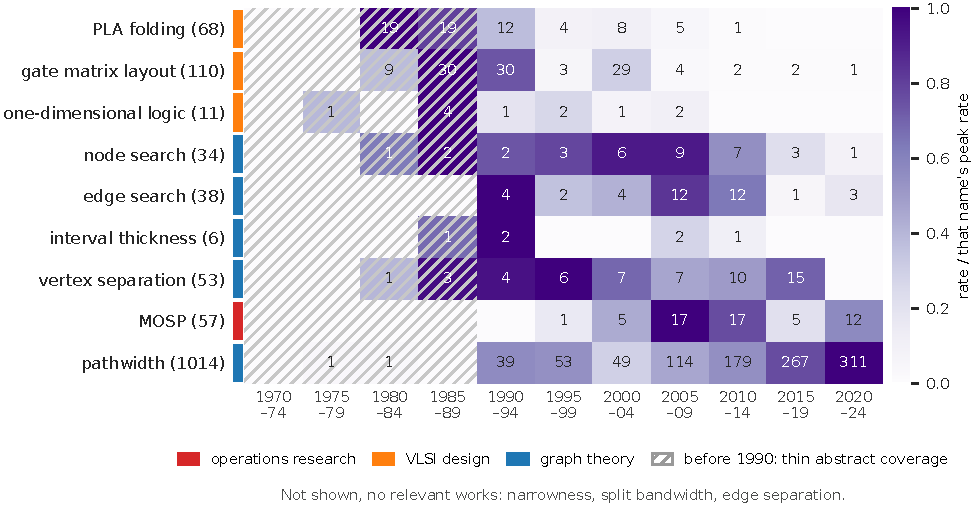
\includegraphics[width=\linewidth]{sec2_fig2_timeline.pdf}
\caption{The VLSI names belong to the 1980s, the search games peak later and
fade, MOSP peaks in 2005--2014, and only pathwidth is still rising. The shade is
the name's rate, relevant works per million works in the same four fields in
each five-year period, as a fraction of that name's own peak rate; the numbers
are raw counts. Rows are ordered by the period of their peak. Counts cover
1970--2024, since 2025--2026 is not fully indexed, so row totals are below those
of Table~\ref{tab:names}. Before 1990 (hatched) OpenAlex has few abstracts.}
\label{fig:timeline}
\end{figure}

\paragraph{When each name was in use.} Figure~\ref{fig:timeline} shows the
counts over time. PLA folding and gate matrix layout peak in 1980--1989 and fall
to almost nothing after 2010, and one-dimensional logic has no relevant work
after 2009. MOSP first appears in the 1990s, peaks in 2005--2014 and is still
active. Pathwidth's rate has roughly doubled since the 1990s, from about 15 to
27 works per million, and its 311 relevant works in 2020--2024 are more than
the whole history of any other name. Rows with a few works per period move by
whole cells on one paper, and should be read as anecdote rather than trend.

% Appendix D: the SAT formulation of MOSP (satisfiability/mosp_encoding.py),
% written 2026-10-09 from the encoder and lean/MOSPFormalization/Encoding.lean.
\section{A SAT formulation of MOSP}
\label{app:sat}

Our SAT formulation encodes the question ``is $Z(M)\le k$?'', for a matrix $M$
with customers $C$ (rows) and patterns $P$ (columns), $m=|P|$, as a formula
in conjunctive normal form, and hands it to a SAT solver; \citet{Knuth2015}
covers the solvers and the encodings used here. It shares no search code and no pruning rule with the customer search of Section~\ref{sec:search}, so it is
an independent check on that search's answers. A satisfying assignment gives a
production order that can be verified by simulation. A refutation can be
logged as a DRAT proof and checked by an independent checker (drat-trim).
Write $P_c$ for the patterns of customer $c$, and positions
$t=0,\dots,m-1$.

\paragraph{Variables.} $x_{p,t}$: pattern $p$ is cut at position $t$.
$y_{p,t}$: pattern $p$ is cut at or before position $t$. $o_{c,t}$: the stack of
customer $c$ is open at position $t$. Two auxiliaries per customer and
position, $\alpha_{c,t}$ (some pattern of $c$ has been cut) and
$\omega_{c,t}$ (all patterns of $c$ have been cut).

\paragraph{Clauses.}
\begin{enumerate}
\item \emph{Permutation.} Every pattern takes at least one position and every
  position at least one pattern, $\bigvee_t x_{p,t}$ and $\bigvee_p x_{p,t}$;
    and at most one of each, by a ladder encoding, shown below.
\item \emph{Prefixes.} $x_{p,t}\Rightarrow y_{p,t}$;
  $y_{p,t}\Rightarrow y_{p,t+1}$; $y_{p,t}\Rightarrow y_{p,t-1}\vee x_{p,t}$
  for $t>0$; and $y_{p,0}\Rightarrow x_{p,0}$.
\item \emph{Open stacks.} A stack is open at $t$ if one of its patterns is cut
  at $t$, $x_{p,t}\Rightarrow o_{c,t}$ for $p\in P_c$, or if some of its
  patterns are cut by $t$ and some are not:
  $y_{p,t}\Rightarrow\alpha_{c,t}$ and $\omega_{c,t}\Rightarrow y_{p,t}$ for
  $p\in P_c$, and $\alpha_{c,t}\wedge\neg\omega_{c,t}\Rightarrow o_{c,t}$.
  These are $2|P_c|+1$ clauses per customer and position instead of the
  $|P_c|(|P_c|-1)$ of the direct pairwise form. Only these polarities are
  needed: no solution gains by setting $o_{c,t}$ true without cause.
\item \emph{Width.} At most $k$ of the $o_{c,t}$ are true at each position $t$,
  by a totalizer.
\item \emph{Symmetry.} Reversing a production order leaves the number of open
  stacks at each step unchanged \citep[Proposition~1]{Yanasse1997a}, so the
  pattern with the most customers may be placed in the first
  $\lfloor m/2\rfloor+1$ positions.
\end{enumerate}

\paragraph{The ladder.} To say that at most one of $z_1,\dots,z_n$ is true,
the ladder introduces auxiliaries $r_1,\dots,r_n$, where $r_i$ reads ``the true
literal, if any, comes after position $i$'', and one slack literal $s$ for
``none is true''. Its clauses are
\[
  r_{i+1}\Rightarrow r_i \ (1\le i<n),\qquad
  z_1\Leftrightarrow\neg r_1,\qquad
  z_i\Leftrightarrow r_{i-1}\wedge\neg r_i \ (1<i\le n),\qquad
  s\Leftrightarrow r_n .
\]
The first family makes $r_1,\dots,r_n$ a ladder, true up to some point and
false after it, so it has exactly one step; the channelling clauses make each
$z_i$ true exactly when the step is at $i$, and $s$ true when there is no step.
So at most one $z_i$ is true, with $n+1$ auxiliaries and about $4n$ clauses,
linear in $n$, where the pairwise form needs $n(n-1)/2$ clauses. Our encoder
emits this form through PySAT's \texttt{EncType.ladder}.

\paragraph{What is proved.} The formula with clauses 1--4 is satisfiable exactly
when some production order keeps at most $k$ stacks open~\leanref{encoding}. The proof models the two cardinality constraints by
their meaning, not by the clauses the ladder and totalizer encodings emit; both
are standard and independent of MOSP. The symmetry clause~5 is justified by the
reversal argument above but is not in the Lean model. That the encoder emits
exactly these clauses is a reading of its source, not a proof.

\paragraph{On the instance of Figure~\ref{fig:wrong}.} The formula has 31,598
variables and 109,923 clauses. Kissat~4.0.4 answers ``satisfiable'' at $k=7$
in 9~s and at $k=6$ in 56~s, with an order whose peak simulates to 6, and
``unsatisfiable'' at $k=5$ in 158~s. CaDiCaL~1.9.5 refutes $k=5$ in 53~s with
a DRAT proof of 1.4 million lemmas (112\,MB compressed), which drat-trim
verifies in 44~s. So the optimum is 6, independently of both versions of the
customer search, with a refutation that a third party can check. The
repository holds the proof trimmed by drat-trim to the lemmas the refutation
uses (27\,MB compressed) and a script that rebuilds the formula from the
instance and checks the proof in about 35~s
(\repofile{paper1/data/false_refutation/drat/}).


\end{document}
